\documentclass[aspectratio=169]{beamer}
% Shared preamble for ml/ slide decks.
% Each lecture .tex starts with:
%   \documentclass[aspectratio=169]{beamer}
%   % Shared preamble for ml/ slide decks.
% Each lecture .tex starts with:
%   \documentclass[aspectratio=169]{beamer}
%   % Shared preamble for ml/ slide decks.
% Each lecture .tex starts with:
%   \documentclass[aspectratio=169]{beamer}
%   \input{../preamble}
% Compile from inside the chapter folder so \input{../preamble} resolves.

\usetheme{default}
\usecolortheme{dove}

\setbeamertemplate{navigation symbols}{}
\setbeamertemplate{footline}{%
  \hfill{\large\insertframenumber\,/\,\inserttotalframenumber}\hspace{0.8em}\vspace{0.5em}%
}

% Project palette (existing, kept for backwards compatibility with deferred/*)
\definecolor{popblue}{RGB}{52, 101, 164}
\definecolor{sampred}{RGB}{204, 0, 0}
\definecolor{paramgreen}{RGB}{0, 140, 70}
\definecolor{warnred}{RGB}{180, 40, 40}
\definecolor{orange1}{RGB}{220, 120, 0}
\definecolor{violet1}{RGB}{120, 50, 160}
\definecolor{lightbg}{RGB}{245, 245, 250}

% Armenian flag palette (use these for any 3-color highlight; per CLAUDE.md).
% "Nice versions": slightly de-saturated from the official spec for slide use,
% so they don't burn out under projector colors. Originals kept as *_pure.
\definecolor{armred}{RGB}{200, 30, 40}      % nice red (official #D90012 muted)
\definecolor{armblue}{RGB}{30, 70, 160}     % nice blue (official #0033A0 muted)
\definecolor{armorange}{RGB}{230, 160, 30}  % nice orange (official #F2A800 muted)
\definecolor{armred_pure}{HTML}{D90012}     % official Armenian flag red
\definecolor{armblue_pure}{HTML}{0033A0}    % official Armenian flag blue
\definecolor{armorange_pure}{HTML}{F2A800}  % official Armenian flag orange

\setbeamercolor{frametitle}{fg=popblue}
\setbeamercolor{title}{fg=popblue}

\usepackage{pgfplots}
\usepackage{tikz}
\usetikzlibrary{shapes, arrows.meta, positioning, calc, decorations.pathreplacing, patterns, matrix}
\pgfplotsset{compat=1.18}
\usepackage{amsmath, amssymb, amsfonts}
\usepackage{bm}
\usepackage{dsfont}
\usepackage{array}
\usepackage{pifont}
\usepackage{colortbl}
\usepackage{fontenc}

% Callout boxes. Purely additive - existing decks are unaffected.
% Usage: \begin{tcolorbox}[colback=armblue!8, colframe=armblue, boxrule=0.6pt, arc=2pt,
%                          title=\textbf{Key idea}] ... \end{tcolorbox}
% Palette convention (ml/SLIDE_STYLE.md): armblue=key idea, armred=trap/warning,
% paramgreen=takeaway or "Next", armorange=watch-out.
\usepackage[most]{tcolorbox}

% Cleaner table rules (\toprule, \midrule, \bottomrule). Also purely additive.
\usepackage{booktabs}

% \cancel{...} for struck-through terms in derivations (added 2026-08-11 for the
% importance-sampling frame in ch11_rl, where the dynamics cancel). Purely additive.
\usepackage{cancel}

% Minimal ML notation macros (subset of slds-lmu latex-math/basic-ml.tex).
% Kept here so we don't have to inline-expand every \thetav, \xv, etc.
% when porting upstream slides.
\newcommand{\R}{\mathds{R}}
\newcommand{\N}{\mathds{N}}
\newcommand{\E}{\mathds{E}}
\newcommand{\Xspace}{\mathcal{X}}
\newcommand{\Yspace}{\mathcal{Y}}
\newcommand{\Hspace}{\mathcal{H}}
\newcommand{\D}{\mathcal{D}}
\newcommand{\Dtrain}{\mathcal{D}_{\text{train}}}
\newcommand{\Dtest}{\mathcal{D}_{\text{test}}}
\newcommand{\xv}{\mathbf{x}}
\newcommand{\yv}{\mathbf{y}}
\newcommand{\Xmat}{\mathbf{X}}
\newcommand{\id}{\mathbf{I}}
\newcommand{\thetav}{\bm{\theta}}
\newcommand{\thetah}{\hat{\bm{\theta}}}
\newcommand{\lamv}{\bm{\lambda}}
\newcommand{\fx}{f(\xv)}
\newcommand{\fxt}{f(\xv \,|\, \bm{\theta})}
\newcommand{\fxi}{f\!\left(\xv^{(i)}\right)}
\newcommand{\fh}{\hat{f}}
\newcommand{\fxh}{\hat{f}(\xv)}
\newcommand{\yh}{\hat{y}}
\newcommand{\yih}{\hat{y}^{(i)}}
% \xi clashes with the Greek letter \xi; write \xv^{(i)} inline instead.
\newcommand{\yi}[1][i]{y^{(#1)}}
\newcommand{\xyi}[1][i]{\left(\xv^{(#1)},\, y^{(#1)}\right)}
\newcommand{\thx}{\bm{\theta}^\top \xv}
\newcommand{\sumin}{\sum_{i=1}^{n}}
\newcommand{\sumjp}{\sum_{j=1}^{p}}
\newcommand{\Lxy}{L\!\left(y, \fx\right)}
\newcommand{\Lxyi}{L\!\left(\yi, \fxi\right)}
\newcommand{\risk}{\mathcal{R}}
\newcommand{\riske}{\mathcal{R}_{\text{emp}}}
\newcommand{\risket}{\mathcal{R}_{\text{emp}}(\bm{\theta})}
\newcommand{\riskt}{\mathcal{R}(\bm{\theta})}
\newcommand{\riskr}{\mathcal{R}_{\text{reg}}}
\newcommand{\argmin}{\mathop{\mathrm{arg\,min}}}
\newcommand{\argmax}{\mathop{\mathrm{arg\,max}}}
\newcommand{\eps}{\varepsilon}

% Compile from inside the chapter folder so % Shared preamble for ml/ slide decks.
% Each lecture .tex starts with:
%   \documentclass[aspectratio=169]{beamer}
%   \input{../preamble}
% Compile from inside the chapter folder so \input{../preamble} resolves.

\usetheme{default}
\usecolortheme{dove}

\setbeamertemplate{navigation symbols}{}
\setbeamertemplate{footline}{%
  \hfill{\large\insertframenumber\,/\,\inserttotalframenumber}\hspace{0.8em}\vspace{0.5em}%
}

% Project palette (existing, kept for backwards compatibility with deferred/*)
\definecolor{popblue}{RGB}{52, 101, 164}
\definecolor{sampred}{RGB}{204, 0, 0}
\definecolor{paramgreen}{RGB}{0, 140, 70}
\definecolor{warnred}{RGB}{180, 40, 40}
\definecolor{orange1}{RGB}{220, 120, 0}
\definecolor{violet1}{RGB}{120, 50, 160}
\definecolor{lightbg}{RGB}{245, 245, 250}

% Armenian flag palette (use these for any 3-color highlight; per CLAUDE.md).
% "Nice versions": slightly de-saturated from the official spec for slide use,
% so they don't burn out under projector colors. Originals kept as *_pure.
\definecolor{armred}{RGB}{200, 30, 40}      % nice red (official #D90012 muted)
\definecolor{armblue}{RGB}{30, 70, 160}     % nice blue (official #0033A0 muted)
\definecolor{armorange}{RGB}{230, 160, 30}  % nice orange (official #F2A800 muted)
\definecolor{armred_pure}{HTML}{D90012}     % official Armenian flag red
\definecolor{armblue_pure}{HTML}{0033A0}    % official Armenian flag blue
\definecolor{armorange_pure}{HTML}{F2A800}  % official Armenian flag orange

\setbeamercolor{frametitle}{fg=popblue}
\setbeamercolor{title}{fg=popblue}

\usepackage{pgfplots}
\usepackage{tikz}
\usetikzlibrary{shapes, arrows.meta, positioning, calc, decorations.pathreplacing, patterns, matrix}
\pgfplotsset{compat=1.18}
\usepackage{amsmath, amssymb, amsfonts}
\usepackage{bm}
\usepackage{dsfont}
\usepackage{array}
\usepackage{pifont}
\usepackage{colortbl}
\usepackage{fontenc}

% Callout boxes. Purely additive - existing decks are unaffected.
% Usage: \begin{tcolorbox}[colback=armblue!8, colframe=armblue, boxrule=0.6pt, arc=2pt,
%                          title=\textbf{Key idea}] ... \end{tcolorbox}
% Palette convention (ml/SLIDE_STYLE.md): armblue=key idea, armred=trap/warning,
% paramgreen=takeaway or "Next", armorange=watch-out.
\usepackage[most]{tcolorbox}

% Cleaner table rules (\toprule, \midrule, \bottomrule). Also purely additive.
\usepackage{booktabs}

% \cancel{...} for struck-through terms in derivations (added 2026-08-11 for the
% importance-sampling frame in ch11_rl, where the dynamics cancel). Purely additive.
\usepackage{cancel}

% Minimal ML notation macros (subset of slds-lmu latex-math/basic-ml.tex).
% Kept here so we don't have to inline-expand every \thetav, \xv, etc.
% when porting upstream slides.
\newcommand{\R}{\mathds{R}}
\newcommand{\N}{\mathds{N}}
\newcommand{\E}{\mathds{E}}
\newcommand{\Xspace}{\mathcal{X}}
\newcommand{\Yspace}{\mathcal{Y}}
\newcommand{\Hspace}{\mathcal{H}}
\newcommand{\D}{\mathcal{D}}
\newcommand{\Dtrain}{\mathcal{D}_{\text{train}}}
\newcommand{\Dtest}{\mathcal{D}_{\text{test}}}
\newcommand{\xv}{\mathbf{x}}
\newcommand{\yv}{\mathbf{y}}
\newcommand{\Xmat}{\mathbf{X}}
\newcommand{\id}{\mathbf{I}}
\newcommand{\thetav}{\bm{\theta}}
\newcommand{\thetah}{\hat{\bm{\theta}}}
\newcommand{\lamv}{\bm{\lambda}}
\newcommand{\fx}{f(\xv)}
\newcommand{\fxt}{f(\xv \,|\, \bm{\theta})}
\newcommand{\fxi}{f\!\left(\xv^{(i)}\right)}
\newcommand{\fh}{\hat{f}}
\newcommand{\fxh}{\hat{f}(\xv)}
\newcommand{\yh}{\hat{y}}
\newcommand{\yih}{\hat{y}^{(i)}}
% \xi clashes with the Greek letter \xi; write \xv^{(i)} inline instead.
\newcommand{\yi}[1][i]{y^{(#1)}}
\newcommand{\xyi}[1][i]{\left(\xv^{(#1)},\, y^{(#1)}\right)}
\newcommand{\thx}{\bm{\theta}^\top \xv}
\newcommand{\sumin}{\sum_{i=1}^{n}}
\newcommand{\sumjp}{\sum_{j=1}^{p}}
\newcommand{\Lxy}{L\!\left(y, \fx\right)}
\newcommand{\Lxyi}{L\!\left(\yi, \fxi\right)}
\newcommand{\risk}{\mathcal{R}}
\newcommand{\riske}{\mathcal{R}_{\text{emp}}}
\newcommand{\risket}{\mathcal{R}_{\text{emp}}(\bm{\theta})}
\newcommand{\riskt}{\mathcal{R}(\bm{\theta})}
\newcommand{\riskr}{\mathcal{R}_{\text{reg}}}
\newcommand{\argmin}{\mathop{\mathrm{arg\,min}}}
\newcommand{\argmax}{\mathop{\mathrm{arg\,max}}}
\newcommand{\eps}{\varepsilon}
 resolves.

\usetheme{default}
\usecolortheme{dove}

\setbeamertemplate{navigation symbols}{}
\setbeamertemplate{footline}{%
  \hfill{\large\insertframenumber\,/\,\inserttotalframenumber}\hspace{0.8em}\vspace{0.5em}%
}

% Project palette (existing, kept for backwards compatibility with deferred/*)
\definecolor{popblue}{RGB}{52, 101, 164}
\definecolor{sampred}{RGB}{204, 0, 0}
\definecolor{paramgreen}{RGB}{0, 140, 70}
\definecolor{warnred}{RGB}{180, 40, 40}
\definecolor{orange1}{RGB}{220, 120, 0}
\definecolor{violet1}{RGB}{120, 50, 160}
\definecolor{lightbg}{RGB}{245, 245, 250}

% Armenian flag palette (use these for any 3-color highlight; per CLAUDE.md).
% "Nice versions": slightly de-saturated from the official spec for slide use,
% so they don't burn out under projector colors. Originals kept as *_pure.
\definecolor{armred}{RGB}{200, 30, 40}      % nice red (official #D90012 muted)
\definecolor{armblue}{RGB}{30, 70, 160}     % nice blue (official #0033A0 muted)
\definecolor{armorange}{RGB}{230, 160, 30}  % nice orange (official #F2A800 muted)
\definecolor{armred_pure}{HTML}{D90012}     % official Armenian flag red
\definecolor{armblue_pure}{HTML}{0033A0}    % official Armenian flag blue
\definecolor{armorange_pure}{HTML}{F2A800}  % official Armenian flag orange

\setbeamercolor{frametitle}{fg=popblue}
\setbeamercolor{title}{fg=popblue}

\usepackage{pgfplots}
\usepackage{tikz}
\usetikzlibrary{shapes, arrows.meta, positioning, calc, decorations.pathreplacing, patterns, matrix}
\pgfplotsset{compat=1.18}
\usepackage{amsmath, amssymb, amsfonts}
\usepackage{bm}
\usepackage{dsfont}
\usepackage{array}
\usepackage{pifont}
\usepackage{colortbl}
\usepackage{fontenc}

% Callout boxes. Purely additive - existing decks are unaffected.
% Usage: \begin{tcolorbox}[colback=armblue!8, colframe=armblue, boxrule=0.6pt, arc=2pt,
%                          title=\textbf{Key idea}] ... \end{tcolorbox}
% Palette convention (ml/SLIDE_STYLE.md): armblue=key idea, armred=trap/warning,
% paramgreen=takeaway or "Next", armorange=watch-out.
\usepackage[most]{tcolorbox}

% Cleaner table rules (\toprule, \midrule, \bottomrule). Also purely additive.
\usepackage{booktabs}

% \cancel{...} for struck-through terms in derivations (added 2026-08-11 for the
% importance-sampling frame in ch11_rl, where the dynamics cancel). Purely additive.
\usepackage{cancel}

% Minimal ML notation macros (subset of slds-lmu latex-math/basic-ml.tex).
% Kept here so we don't have to inline-expand every \thetav, \xv, etc.
% when porting upstream slides.
\newcommand{\R}{\mathds{R}}
\newcommand{\N}{\mathds{N}}
\newcommand{\E}{\mathds{E}}
\newcommand{\Xspace}{\mathcal{X}}
\newcommand{\Yspace}{\mathcal{Y}}
\newcommand{\Hspace}{\mathcal{H}}
\newcommand{\D}{\mathcal{D}}
\newcommand{\Dtrain}{\mathcal{D}_{\text{train}}}
\newcommand{\Dtest}{\mathcal{D}_{\text{test}}}
\newcommand{\xv}{\mathbf{x}}
\newcommand{\yv}{\mathbf{y}}
\newcommand{\Xmat}{\mathbf{X}}
\newcommand{\id}{\mathbf{I}}
\newcommand{\thetav}{\bm{\theta}}
\newcommand{\thetah}{\hat{\bm{\theta}}}
\newcommand{\lamv}{\bm{\lambda}}
\newcommand{\fx}{f(\xv)}
\newcommand{\fxt}{f(\xv \,|\, \bm{\theta})}
\newcommand{\fxi}{f\!\left(\xv^{(i)}\right)}
\newcommand{\fh}{\hat{f}}
\newcommand{\fxh}{\hat{f}(\xv)}
\newcommand{\yh}{\hat{y}}
\newcommand{\yih}{\hat{y}^{(i)}}
% \xi clashes with the Greek letter \xi; write \xv^{(i)} inline instead.
\newcommand{\yi}[1][i]{y^{(#1)}}
\newcommand{\xyi}[1][i]{\left(\xv^{(#1)},\, y^{(#1)}\right)}
\newcommand{\thx}{\bm{\theta}^\top \xv}
\newcommand{\sumin}{\sum_{i=1}^{n}}
\newcommand{\sumjp}{\sum_{j=1}^{p}}
\newcommand{\Lxy}{L\!\left(y, \fx\right)}
\newcommand{\Lxyi}{L\!\left(\yi, \fxi\right)}
\newcommand{\risk}{\mathcal{R}}
\newcommand{\riske}{\mathcal{R}_{\text{emp}}}
\newcommand{\risket}{\mathcal{R}_{\text{emp}}(\bm{\theta})}
\newcommand{\riskt}{\mathcal{R}(\bm{\theta})}
\newcommand{\riskr}{\mathcal{R}_{\text{reg}}}
\newcommand{\argmin}{\mathop{\mathrm{arg\,min}}}
\newcommand{\argmax}{\mathop{\mathrm{arg\,max}}}
\newcommand{\eps}{\varepsilon}

% Compile from inside the chapter folder so % Shared preamble for ml/ slide decks.
% Each lecture .tex starts with:
%   \documentclass[aspectratio=169]{beamer}
%   % Shared preamble for ml/ slide decks.
% Each lecture .tex starts with:
%   \documentclass[aspectratio=169]{beamer}
%   \input{../preamble}
% Compile from inside the chapter folder so \input{../preamble} resolves.

\usetheme{default}
\usecolortheme{dove}

\setbeamertemplate{navigation symbols}{}
\setbeamertemplate{footline}{%
  \hfill{\large\insertframenumber\,/\,\inserttotalframenumber}\hspace{0.8em}\vspace{0.5em}%
}

% Project palette (existing, kept for backwards compatibility with deferred/*)
\definecolor{popblue}{RGB}{52, 101, 164}
\definecolor{sampred}{RGB}{204, 0, 0}
\definecolor{paramgreen}{RGB}{0, 140, 70}
\definecolor{warnred}{RGB}{180, 40, 40}
\definecolor{orange1}{RGB}{220, 120, 0}
\definecolor{violet1}{RGB}{120, 50, 160}
\definecolor{lightbg}{RGB}{245, 245, 250}

% Armenian flag palette (use these for any 3-color highlight; per CLAUDE.md).
% "Nice versions": slightly de-saturated from the official spec for slide use,
% so they don't burn out under projector colors. Originals kept as *_pure.
\definecolor{armred}{RGB}{200, 30, 40}      % nice red (official #D90012 muted)
\definecolor{armblue}{RGB}{30, 70, 160}     % nice blue (official #0033A0 muted)
\definecolor{armorange}{RGB}{230, 160, 30}  % nice orange (official #F2A800 muted)
\definecolor{armred_pure}{HTML}{D90012}     % official Armenian flag red
\definecolor{armblue_pure}{HTML}{0033A0}    % official Armenian flag blue
\definecolor{armorange_pure}{HTML}{F2A800}  % official Armenian flag orange

\setbeamercolor{frametitle}{fg=popblue}
\setbeamercolor{title}{fg=popblue}

\usepackage{pgfplots}
\usepackage{tikz}
\usetikzlibrary{shapes, arrows.meta, positioning, calc, decorations.pathreplacing, patterns, matrix}
\pgfplotsset{compat=1.18}
\usepackage{amsmath, amssymb, amsfonts}
\usepackage{bm}
\usepackage{dsfont}
\usepackage{array}
\usepackage{pifont}
\usepackage{colortbl}
\usepackage{fontenc}

% Callout boxes. Purely additive - existing decks are unaffected.
% Usage: \begin{tcolorbox}[colback=armblue!8, colframe=armblue, boxrule=0.6pt, arc=2pt,
%                          title=\textbf{Key idea}] ... \end{tcolorbox}
% Palette convention (ml/SLIDE_STYLE.md): armblue=key idea, armred=trap/warning,
% paramgreen=takeaway or "Next", armorange=watch-out.
\usepackage[most]{tcolorbox}

% Cleaner table rules (\toprule, \midrule, \bottomrule). Also purely additive.
\usepackage{booktabs}

% \cancel{...} for struck-through terms in derivations (added 2026-08-11 for the
% importance-sampling frame in ch11_rl, where the dynamics cancel). Purely additive.
\usepackage{cancel}

% Minimal ML notation macros (subset of slds-lmu latex-math/basic-ml.tex).
% Kept here so we don't have to inline-expand every \thetav, \xv, etc.
% when porting upstream slides.
\newcommand{\R}{\mathds{R}}
\newcommand{\N}{\mathds{N}}
\newcommand{\E}{\mathds{E}}
\newcommand{\Xspace}{\mathcal{X}}
\newcommand{\Yspace}{\mathcal{Y}}
\newcommand{\Hspace}{\mathcal{H}}
\newcommand{\D}{\mathcal{D}}
\newcommand{\Dtrain}{\mathcal{D}_{\text{train}}}
\newcommand{\Dtest}{\mathcal{D}_{\text{test}}}
\newcommand{\xv}{\mathbf{x}}
\newcommand{\yv}{\mathbf{y}}
\newcommand{\Xmat}{\mathbf{X}}
\newcommand{\id}{\mathbf{I}}
\newcommand{\thetav}{\bm{\theta}}
\newcommand{\thetah}{\hat{\bm{\theta}}}
\newcommand{\lamv}{\bm{\lambda}}
\newcommand{\fx}{f(\xv)}
\newcommand{\fxt}{f(\xv \,|\, \bm{\theta})}
\newcommand{\fxi}{f\!\left(\xv^{(i)}\right)}
\newcommand{\fh}{\hat{f}}
\newcommand{\fxh}{\hat{f}(\xv)}
\newcommand{\yh}{\hat{y}}
\newcommand{\yih}{\hat{y}^{(i)}}
% \xi clashes with the Greek letter \xi; write \xv^{(i)} inline instead.
\newcommand{\yi}[1][i]{y^{(#1)}}
\newcommand{\xyi}[1][i]{\left(\xv^{(#1)},\, y^{(#1)}\right)}
\newcommand{\thx}{\bm{\theta}^\top \xv}
\newcommand{\sumin}{\sum_{i=1}^{n}}
\newcommand{\sumjp}{\sum_{j=1}^{p}}
\newcommand{\Lxy}{L\!\left(y, \fx\right)}
\newcommand{\Lxyi}{L\!\left(\yi, \fxi\right)}
\newcommand{\risk}{\mathcal{R}}
\newcommand{\riske}{\mathcal{R}_{\text{emp}}}
\newcommand{\risket}{\mathcal{R}_{\text{emp}}(\bm{\theta})}
\newcommand{\riskt}{\mathcal{R}(\bm{\theta})}
\newcommand{\riskr}{\mathcal{R}_{\text{reg}}}
\newcommand{\argmin}{\mathop{\mathrm{arg\,min}}}
\newcommand{\argmax}{\mathop{\mathrm{arg\,max}}}
\newcommand{\eps}{\varepsilon}

% Compile from inside the chapter folder so % Shared preamble for ml/ slide decks.
% Each lecture .tex starts with:
%   \documentclass[aspectratio=169]{beamer}
%   \input{../preamble}
% Compile from inside the chapter folder so \input{../preamble} resolves.

\usetheme{default}
\usecolortheme{dove}

\setbeamertemplate{navigation symbols}{}
\setbeamertemplate{footline}{%
  \hfill{\large\insertframenumber\,/\,\inserttotalframenumber}\hspace{0.8em}\vspace{0.5em}%
}

% Project palette (existing, kept for backwards compatibility with deferred/*)
\definecolor{popblue}{RGB}{52, 101, 164}
\definecolor{sampred}{RGB}{204, 0, 0}
\definecolor{paramgreen}{RGB}{0, 140, 70}
\definecolor{warnred}{RGB}{180, 40, 40}
\definecolor{orange1}{RGB}{220, 120, 0}
\definecolor{violet1}{RGB}{120, 50, 160}
\definecolor{lightbg}{RGB}{245, 245, 250}

% Armenian flag palette (use these for any 3-color highlight; per CLAUDE.md).
% "Nice versions": slightly de-saturated from the official spec for slide use,
% so they don't burn out under projector colors. Originals kept as *_pure.
\definecolor{armred}{RGB}{200, 30, 40}      % nice red (official #D90012 muted)
\definecolor{armblue}{RGB}{30, 70, 160}     % nice blue (official #0033A0 muted)
\definecolor{armorange}{RGB}{230, 160, 30}  % nice orange (official #F2A800 muted)
\definecolor{armred_pure}{HTML}{D90012}     % official Armenian flag red
\definecolor{armblue_pure}{HTML}{0033A0}    % official Armenian flag blue
\definecolor{armorange_pure}{HTML}{F2A800}  % official Armenian flag orange

\setbeamercolor{frametitle}{fg=popblue}
\setbeamercolor{title}{fg=popblue}

\usepackage{pgfplots}
\usepackage{tikz}
\usetikzlibrary{shapes, arrows.meta, positioning, calc, decorations.pathreplacing, patterns, matrix}
\pgfplotsset{compat=1.18}
\usepackage{amsmath, amssymb, amsfonts}
\usepackage{bm}
\usepackage{dsfont}
\usepackage{array}
\usepackage{pifont}
\usepackage{colortbl}
\usepackage{fontenc}

% Callout boxes. Purely additive - existing decks are unaffected.
% Usage: \begin{tcolorbox}[colback=armblue!8, colframe=armblue, boxrule=0.6pt, arc=2pt,
%                          title=\textbf{Key idea}] ... \end{tcolorbox}
% Palette convention (ml/SLIDE_STYLE.md): armblue=key idea, armred=trap/warning,
% paramgreen=takeaway or "Next", armorange=watch-out.
\usepackage[most]{tcolorbox}

% Cleaner table rules (\toprule, \midrule, \bottomrule). Also purely additive.
\usepackage{booktabs}

% \cancel{...} for struck-through terms in derivations (added 2026-08-11 for the
% importance-sampling frame in ch11_rl, where the dynamics cancel). Purely additive.
\usepackage{cancel}

% Minimal ML notation macros (subset of slds-lmu latex-math/basic-ml.tex).
% Kept here so we don't have to inline-expand every \thetav, \xv, etc.
% when porting upstream slides.
\newcommand{\R}{\mathds{R}}
\newcommand{\N}{\mathds{N}}
\newcommand{\E}{\mathds{E}}
\newcommand{\Xspace}{\mathcal{X}}
\newcommand{\Yspace}{\mathcal{Y}}
\newcommand{\Hspace}{\mathcal{H}}
\newcommand{\D}{\mathcal{D}}
\newcommand{\Dtrain}{\mathcal{D}_{\text{train}}}
\newcommand{\Dtest}{\mathcal{D}_{\text{test}}}
\newcommand{\xv}{\mathbf{x}}
\newcommand{\yv}{\mathbf{y}}
\newcommand{\Xmat}{\mathbf{X}}
\newcommand{\id}{\mathbf{I}}
\newcommand{\thetav}{\bm{\theta}}
\newcommand{\thetah}{\hat{\bm{\theta}}}
\newcommand{\lamv}{\bm{\lambda}}
\newcommand{\fx}{f(\xv)}
\newcommand{\fxt}{f(\xv \,|\, \bm{\theta})}
\newcommand{\fxi}{f\!\left(\xv^{(i)}\right)}
\newcommand{\fh}{\hat{f}}
\newcommand{\fxh}{\hat{f}(\xv)}
\newcommand{\yh}{\hat{y}}
\newcommand{\yih}{\hat{y}^{(i)}}
% \xi clashes with the Greek letter \xi; write \xv^{(i)} inline instead.
\newcommand{\yi}[1][i]{y^{(#1)}}
\newcommand{\xyi}[1][i]{\left(\xv^{(#1)},\, y^{(#1)}\right)}
\newcommand{\thx}{\bm{\theta}^\top \xv}
\newcommand{\sumin}{\sum_{i=1}^{n}}
\newcommand{\sumjp}{\sum_{j=1}^{p}}
\newcommand{\Lxy}{L\!\left(y, \fx\right)}
\newcommand{\Lxyi}{L\!\left(\yi, \fxi\right)}
\newcommand{\risk}{\mathcal{R}}
\newcommand{\riske}{\mathcal{R}_{\text{emp}}}
\newcommand{\risket}{\mathcal{R}_{\text{emp}}(\bm{\theta})}
\newcommand{\riskt}{\mathcal{R}(\bm{\theta})}
\newcommand{\riskr}{\mathcal{R}_{\text{reg}}}
\newcommand{\argmin}{\mathop{\mathrm{arg\,min}}}
\newcommand{\argmax}{\mathop{\mathrm{arg\,max}}}
\newcommand{\eps}{\varepsilon}
 resolves.

\usetheme{default}
\usecolortheme{dove}

\setbeamertemplate{navigation symbols}{}
\setbeamertemplate{footline}{%
  \hfill{\large\insertframenumber\,/\,\inserttotalframenumber}\hspace{0.8em}\vspace{0.5em}%
}

% Project palette (existing, kept for backwards compatibility with deferred/*)
\definecolor{popblue}{RGB}{52, 101, 164}
\definecolor{sampred}{RGB}{204, 0, 0}
\definecolor{paramgreen}{RGB}{0, 140, 70}
\definecolor{warnred}{RGB}{180, 40, 40}
\definecolor{orange1}{RGB}{220, 120, 0}
\definecolor{violet1}{RGB}{120, 50, 160}
\definecolor{lightbg}{RGB}{245, 245, 250}

% Armenian flag palette (use these for any 3-color highlight; per CLAUDE.md).
% "Nice versions": slightly de-saturated from the official spec for slide use,
% so they don't burn out under projector colors. Originals kept as *_pure.
\definecolor{armred}{RGB}{200, 30, 40}      % nice red (official #D90012 muted)
\definecolor{armblue}{RGB}{30, 70, 160}     % nice blue (official #0033A0 muted)
\definecolor{armorange}{RGB}{230, 160, 30}  % nice orange (official #F2A800 muted)
\definecolor{armred_pure}{HTML}{D90012}     % official Armenian flag red
\definecolor{armblue_pure}{HTML}{0033A0}    % official Armenian flag blue
\definecolor{armorange_pure}{HTML}{F2A800}  % official Armenian flag orange

\setbeamercolor{frametitle}{fg=popblue}
\setbeamercolor{title}{fg=popblue}

\usepackage{pgfplots}
\usepackage{tikz}
\usetikzlibrary{shapes, arrows.meta, positioning, calc, decorations.pathreplacing, patterns, matrix}
\pgfplotsset{compat=1.18}
\usepackage{amsmath, amssymb, amsfonts}
\usepackage{bm}
\usepackage{dsfont}
\usepackage{array}
\usepackage{pifont}
\usepackage{colortbl}
\usepackage{fontenc}

% Callout boxes. Purely additive - existing decks are unaffected.
% Usage: \begin{tcolorbox}[colback=armblue!8, colframe=armblue, boxrule=0.6pt, arc=2pt,
%                          title=\textbf{Key idea}] ... \end{tcolorbox}
% Palette convention (ml/SLIDE_STYLE.md): armblue=key idea, armred=trap/warning,
% paramgreen=takeaway or "Next", armorange=watch-out.
\usepackage[most]{tcolorbox}

% Cleaner table rules (\toprule, \midrule, \bottomrule). Also purely additive.
\usepackage{booktabs}

% \cancel{...} for struck-through terms in derivations (added 2026-08-11 for the
% importance-sampling frame in ch11_rl, where the dynamics cancel). Purely additive.
\usepackage{cancel}

% Minimal ML notation macros (subset of slds-lmu latex-math/basic-ml.tex).
% Kept here so we don't have to inline-expand every \thetav, \xv, etc.
% when porting upstream slides.
\newcommand{\R}{\mathds{R}}
\newcommand{\N}{\mathds{N}}
\newcommand{\E}{\mathds{E}}
\newcommand{\Xspace}{\mathcal{X}}
\newcommand{\Yspace}{\mathcal{Y}}
\newcommand{\Hspace}{\mathcal{H}}
\newcommand{\D}{\mathcal{D}}
\newcommand{\Dtrain}{\mathcal{D}_{\text{train}}}
\newcommand{\Dtest}{\mathcal{D}_{\text{test}}}
\newcommand{\xv}{\mathbf{x}}
\newcommand{\yv}{\mathbf{y}}
\newcommand{\Xmat}{\mathbf{X}}
\newcommand{\id}{\mathbf{I}}
\newcommand{\thetav}{\bm{\theta}}
\newcommand{\thetah}{\hat{\bm{\theta}}}
\newcommand{\lamv}{\bm{\lambda}}
\newcommand{\fx}{f(\xv)}
\newcommand{\fxt}{f(\xv \,|\, \bm{\theta})}
\newcommand{\fxi}{f\!\left(\xv^{(i)}\right)}
\newcommand{\fh}{\hat{f}}
\newcommand{\fxh}{\hat{f}(\xv)}
\newcommand{\yh}{\hat{y}}
\newcommand{\yih}{\hat{y}^{(i)}}
% \xi clashes with the Greek letter \xi; write \xv^{(i)} inline instead.
\newcommand{\yi}[1][i]{y^{(#1)}}
\newcommand{\xyi}[1][i]{\left(\xv^{(#1)},\, y^{(#1)}\right)}
\newcommand{\thx}{\bm{\theta}^\top \xv}
\newcommand{\sumin}{\sum_{i=1}^{n}}
\newcommand{\sumjp}{\sum_{j=1}^{p}}
\newcommand{\Lxy}{L\!\left(y, \fx\right)}
\newcommand{\Lxyi}{L\!\left(\yi, \fxi\right)}
\newcommand{\risk}{\mathcal{R}}
\newcommand{\riske}{\mathcal{R}_{\text{emp}}}
\newcommand{\risket}{\mathcal{R}_{\text{emp}}(\bm{\theta})}
\newcommand{\riskt}{\mathcal{R}(\bm{\theta})}
\newcommand{\riskr}{\mathcal{R}_{\text{reg}}}
\newcommand{\argmin}{\mathop{\mathrm{arg\,min}}}
\newcommand{\argmax}{\mathop{\mathrm{arg\,max}}}
\newcommand{\eps}{\varepsilon}
 resolves.

\usetheme{default}
\usecolortheme{dove}

\setbeamertemplate{navigation symbols}{}
\setbeamertemplate{footline}{%
  \hfill{\large\insertframenumber\,/\,\inserttotalframenumber}\hspace{0.8em}\vspace{0.5em}%
}

% Project palette (existing, kept for backwards compatibility with deferred/*)
\definecolor{popblue}{RGB}{52, 101, 164}
\definecolor{sampred}{RGB}{204, 0, 0}
\definecolor{paramgreen}{RGB}{0, 140, 70}
\definecolor{warnred}{RGB}{180, 40, 40}
\definecolor{orange1}{RGB}{220, 120, 0}
\definecolor{violet1}{RGB}{120, 50, 160}
\definecolor{lightbg}{RGB}{245, 245, 250}

% Armenian flag palette (use these for any 3-color highlight; per CLAUDE.md).
% "Nice versions": slightly de-saturated from the official spec for slide use,
% so they don't burn out under projector colors. Originals kept as *_pure.
\definecolor{armred}{RGB}{200, 30, 40}      % nice red (official #D90012 muted)
\definecolor{armblue}{RGB}{30, 70, 160}     % nice blue (official #0033A0 muted)
\definecolor{armorange}{RGB}{230, 160, 30}  % nice orange (official #F2A800 muted)
\definecolor{armred_pure}{HTML}{D90012}     % official Armenian flag red
\definecolor{armblue_pure}{HTML}{0033A0}    % official Armenian flag blue
\definecolor{armorange_pure}{HTML}{F2A800}  % official Armenian flag orange

\setbeamercolor{frametitle}{fg=popblue}
\setbeamercolor{title}{fg=popblue}

\usepackage{pgfplots}
\usepackage{tikz}
\usetikzlibrary{shapes, arrows.meta, positioning, calc, decorations.pathreplacing, patterns, matrix}
\pgfplotsset{compat=1.18}
\usepackage{amsmath, amssymb, amsfonts}
\usepackage{bm}
\usepackage{dsfont}
\usepackage{array}
\usepackage{pifont}
\usepackage{colortbl}
\usepackage{fontenc}

% Callout boxes. Purely additive - existing decks are unaffected.
% Usage: \begin{tcolorbox}[colback=armblue!8, colframe=armblue, boxrule=0.6pt, arc=2pt,
%                          title=\textbf{Key idea}] ... \end{tcolorbox}
% Palette convention (ml/SLIDE_STYLE.md): armblue=key idea, armred=trap/warning,
% paramgreen=takeaway or "Next", armorange=watch-out.
\usepackage[most]{tcolorbox}

% Cleaner table rules (\toprule, \midrule, \bottomrule). Also purely additive.
\usepackage{booktabs}

% \cancel{...} for struck-through terms in derivations (added 2026-08-11 for the
% importance-sampling frame in ch11_rl, where the dynamics cancel). Purely additive.
\usepackage{cancel}

% Minimal ML notation macros (subset of slds-lmu latex-math/basic-ml.tex).
% Kept here so we don't have to inline-expand every \thetav, \xv, etc.
% when porting upstream slides.
\newcommand{\R}{\mathds{R}}
\newcommand{\N}{\mathds{N}}
\newcommand{\E}{\mathds{E}}
\newcommand{\Xspace}{\mathcal{X}}
\newcommand{\Yspace}{\mathcal{Y}}
\newcommand{\Hspace}{\mathcal{H}}
\newcommand{\D}{\mathcal{D}}
\newcommand{\Dtrain}{\mathcal{D}_{\text{train}}}
\newcommand{\Dtest}{\mathcal{D}_{\text{test}}}
\newcommand{\xv}{\mathbf{x}}
\newcommand{\yv}{\mathbf{y}}
\newcommand{\Xmat}{\mathbf{X}}
\newcommand{\id}{\mathbf{I}}
\newcommand{\thetav}{\bm{\theta}}
\newcommand{\thetah}{\hat{\bm{\theta}}}
\newcommand{\lamv}{\bm{\lambda}}
\newcommand{\fx}{f(\xv)}
\newcommand{\fxt}{f(\xv \,|\, \bm{\theta})}
\newcommand{\fxi}{f\!\left(\xv^{(i)}\right)}
\newcommand{\fh}{\hat{f}}
\newcommand{\fxh}{\hat{f}(\xv)}
\newcommand{\yh}{\hat{y}}
\newcommand{\yih}{\hat{y}^{(i)}}
% \xi clashes with the Greek letter \xi; write \xv^{(i)} inline instead.
\newcommand{\yi}[1][i]{y^{(#1)}}
\newcommand{\xyi}[1][i]{\left(\xv^{(#1)},\, y^{(#1)}\right)}
\newcommand{\thx}{\bm{\theta}^\top \xv}
\newcommand{\sumin}{\sum_{i=1}^{n}}
\newcommand{\sumjp}{\sum_{j=1}^{p}}
\newcommand{\Lxy}{L\!\left(y, \fx\right)}
\newcommand{\Lxyi}{L\!\left(\yi, \fxi\right)}
\newcommand{\risk}{\mathcal{R}}
\newcommand{\riske}{\mathcal{R}_{\text{emp}}}
\newcommand{\risket}{\mathcal{R}_{\text{emp}}(\bm{\theta})}
\newcommand{\riskt}{\mathcal{R}(\bm{\theta})}
\newcommand{\riskr}{\mathcal{R}_{\text{reg}}}
\newcommand{\argmin}{\mathop{\mathrm{arg\,min}}}
\newcommand{\argmax}{\mathop{\mathrm{arg\,max}}}
\newcommand{\eps}{\varepsilon}


\graphicspath{{fig/}{fig/borrowed/}}

\title{RNN Foundations}
\subtitle{Networks with memory - and why the memory fades}
\date{}

\begin{document}

\begin{frame}
  \titlepage
  \begin{center}\scriptsize\color{gray}
    Parts of this chapter adapt LMU I2DL (slds-lmu), CC BY 4.0.
  \end{center}
\end{frame}

% ================================================================
% COLD OPEN
\begin{frame}{The reviews arrive}
  \begin{columns}[T]
    \column{0.52\textwidth}
    \small
    The [50] classifier grades each pomegranate; the boxes ship worldwide. Now the
    \textbf{reviews} arrive: "Fresh and sweet!" (3 words); an 11-word one naming Yerevan;
    a 42-word complaint; some in Armenian. Ops wants them read, translated, answered.
    \vskip 3pt
    Zoom out: \textbf{every} headline AI system of the 2020s - ChatGPT included - is a
    \textbf{sequence model}. This chapter and the next are the road there.
    \vskip 4pt
    \textbf{Predict:} feed a review into an MLP ([41\_2]) - what breaks before you even
    train?
    \pause
    \vskip 3pt
    \fcolorbox{armred}{armred!8}{\parbox{0.95\linewidth}{\small
      The input layer has a \textbf{fixed size}. Reviews do not.}}
    \column{0.48\textwidth}
    \begin{center}
      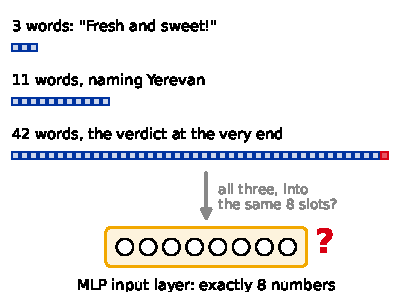
\includegraphics[width=\linewidth]{cold_open.pdf}
    \end{center}
  \end{columns}
\end{frame}

\begin{frame}{Outline}
  \tableofcontents
\end{frame}

% ================================================================
\section{Text refuses to fit}

\begin{frame}[plain]
  \vfill
  \begin{center}
    {\Large\color{popblue}\textbf{Text refuses to fit}}\\[0.9em]
    \begin{minipage}{0.82\textwidth}\centering\small
      Order is information, and length is a variable.
    \end{minipage}
  \end{center}
  \vfill
\end{frame}

% 2026-10-15: time series replaced by speech and music (instructor), and the three text
% boxes replaced by a figure that shows each kind of sequence (l20_diagrams.py).
\begin{frame}{The sequence zoo}
  \begin{columns}[T]
    \column{0.40\textwidth}
    \small
    Text leads this chapter. Two close cousins share the same shape of problem:
    \textbf{speech} (a voice is a long list of air-pressure numbers) and \textbf{music}
    (a melody is a list of notes).
    \vskip 6pt
    \fcolorbox{armblue}{armblue!8}{\parbox{0.95\linewidth}{\raggedright\small
      What they share: \textbf{order matters}, \textbf{length varies}, and dependencies
      can be \textbf{long-range} - the word that resolves a sentence's meaning may be
      40 tokens back.}}
    \column{0.60\textwidth}
    \begin{center}
      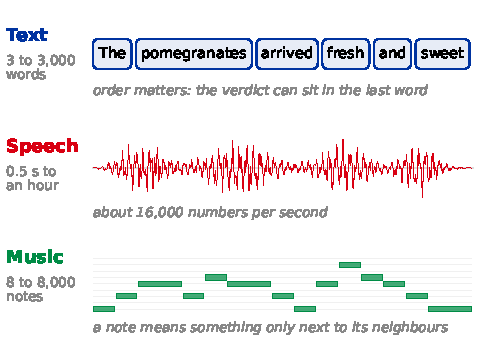
\includegraphics[width=\linewidth]{seq_zoo.pdf}
    \end{center}
  \end{columns}
\end{frame}

\begin{frame}{The shuffle test}
  \begin{columns}[T]
    \column{0.30\textwidth}
    Take the review sentence and shuffle its words with one fixed permutation. Every
    word is identical; all meaning is gone.
    \vskip 6pt
    \fcolorbox{armred}{armred!8}{\parbox{0.95\linewidth}{\raggedright\small
      The bag-of-words histograms are \textbf{pixel-identical}. Any order-blind model
      literally cannot tell the two apart.}}
    \vskip 6pt
    {\footnotesize Callback: [48] did this to an image's \emph{pixels}. Same demo, new
    axis.}
    \column{0.70\textwidth}
    \begin{center}
      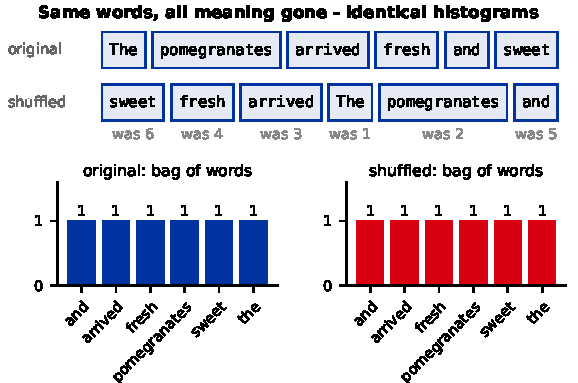
\includegraphics[width=\linewidth]{word_shuffle.pdf}
    \end{center}
  \end{columns}
\end{frame}

\begin{frame}{The shoehorn hacks}
  How people force variable-length text into a fixed net - and the price of each:
  \begin{center}
    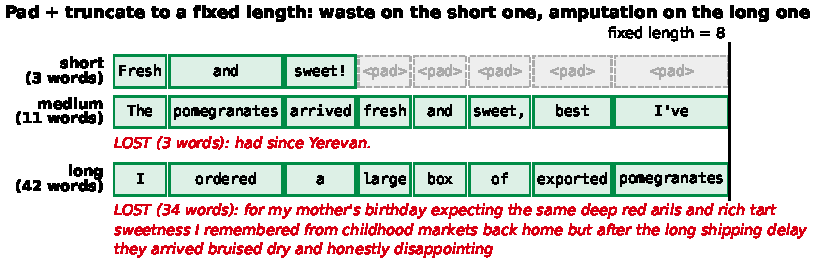
\includegraphics[width=\linewidth]{pad_truncate.pdf}
  \end{center}
  \fcolorbox{armorange}{armorange!12}{\parbox{0.97\linewidth}{\small
      \textbf{(2) Bag-of-words averaging} fails the shuffle test by construction - it
      cannot see order at all. \textbf{(3) A separate weight per position} means "I went
      to Munich in 2009" and "In 2009, I went to Munich" must each relearn the same fact
      at a different position.}}
\end{frame}

% 2026-09-22 addition: the bridge from L19 (1D conv on text) and the ch11 name inventor
% (Bengio-style fixed-context MLP) - "why not just a window?" was never asked.
\begin{frame}{What about a fixed window?}
  \small
  You have already met two models that read a sequence through a \textbf{fixed window}
  of the last $k$ tokens:
  \begin{itemize}
    \item the \textbf{1D convolution} from [48] - slide the same kernel along a sentence
      instead of a signal, and it reads a window of $k$ tokens;
    \item the ch11 \textbf{name inventor} - an MLP that predicts the next letter from the
      last $k$ letters (Bengio et al., 2003).
  \end{itemize}
  Both learn \textbf{local} patterns well - "-yan" closes an Armenian surname. Both are
  \textbf{blind beyond $k$}:
  \vskip 6pt
  \begin{center}
    The \textbf{pomegranates} that my grandmother sent us
    \colorbox{armorange!30}{from Goris last autumn} \textbf{were} sweet.
  \end{center}
  \vskip 2pt
  A 4-word window in front of "were" sees only \emph{from Goris last autumn}. It cannot
  tell whether one pomegranate or many was sent - the word that decides it is 10 words
  back.
  \vskip 6pt
  \fcolorbox{armblue}{armblue!8}{\parbox{0.97\linewidth}{\small
    Stacking conv layers widens the window ([49]'s receptive field), but the width is
    fixed by the architecture before any text arrives. We want a memory that grows
    \emph{with} the text: read one token at a time and carry a summary forward.}}
\end{frame}

\begin{frame}{Tokens, minimally}
  \begin{columns}[T]
    \column{0.36\textwidth}
    To feed text to \emph{any} network, words must first become vectors. For now, the
    simplest scheme: build a \textbf{vocabulary}, then represent each word as a
    \textbf{one-hot} vector.
    \vskip 6pt
    \fcolorbox{armblue}{armblue!8}{\parbox{0.95\linewidth}{\small
      Callback: [03] one-hot encoded categorical features. Same trick, new victim - a
      \emph{word} instead of a category.}}
    \vskip 6pt
    {\footnotesize The full tokenization story (subwords, vocabulary explosion, the
    Armenian fact) comes in the LLM chapter.}
    \column{0.64\textwidth}
    \begin{center}
      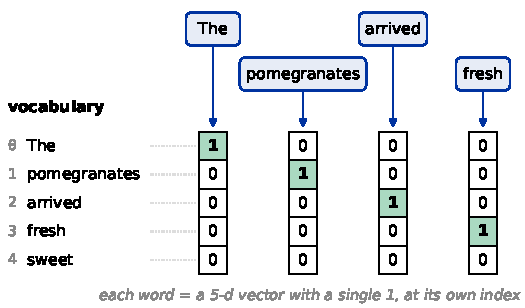
\includegraphics[width=\linewidth]{onehot_columns.pdf}
    \end{center}
  \end{columns}
\end{frame}

% 2026-10-03: moved here from L21 (its tokenization section moved to the LLM chapter).
\begin{frame}{One-hot and its poverty}
  \begin{columns}[T]
    \column{0.42\textwidth}
    \small
    One-hot is all this chapter needs. It has one flaw worth seeing now:
    \vskip 6pt
    \fcolorbox{armred}{armred!8}{\parbox{0.95\linewidth}{\raggedright\small
      In a 10,000-dimensional one-hot space, \textbf{every pair of words is equally
      far apart}. "good" is as far from "great" as it is from "plastic" - the
      geometry carries zero meaning.}}
    \vskip 6pt
    {\footnotesize With 3 words it fits in a picture: the words are the 3 corners of a cube
    next to the origin, and every edge between them is $\sqrt{2}$ long. Learned, dense word
    vectors fix this. They arrive with the attention chapter.}
    \column{0.58\textwidth}
    \begin{center}
      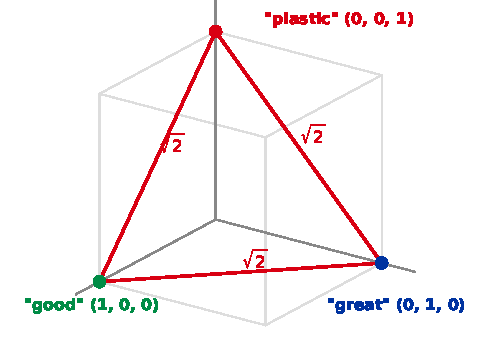
\includegraphics[width=\linewidth]{onehot_cube.pdf}
    \end{center}
  \end{columns}
\end{frame}

% ================================================================
\section{The recurrence idea}

\begin{frame}[plain]
  \vfill
  \begin{center}
    {\Large\color{popblue}\textbf{The recurrence idea}}\\[0.9em]
    \begin{minipage}{0.82\textwidth}\centering\small
      Read like a human: one word at a time, with memory.
    \end{minipage}
  \end{center}
  \vfill
\end{frame}

% 2026-10-03: on-ramp from [29] (instructor-approved). The 0.8 here is paid off in
% "Predict-first: the fading number". Weights checked: 0.2 * 0.8^k = 0.20, 0.16, 0.128, 0.1024.
\begin{frame}{You have already run a recurrence}
  \begin{columns}[T]
    \column{0.47\textwidth}
    \small
    [29]'s \textbf{exponential smoothing} forecast tomorrow from a running summary of the
    whole past:
    \[
      \hat{y}_{t+1} = \alpha\, y_t + (1-\alpha)\,\hat{y}_t
    \]
    New summary $=$ a little of today $+$ most of the old summary. Unroll it and each older
    reading's weight shrinks by the same factor every step: with $\alpha = 0.2$ the weights
    are $0.20, 0.16, 0.13, 0.10, \dots$ - each one $0.8$ of the one before.
    \column{0.53\textwidth}
    \vskip 2pt
    \footnotesize
    \begin{tabular}{@{}lll@{}}
      & \textbf{smoothing, [29]} & \textbf{RNN, today} \\[2pt]
      \hline\\[-8pt]
      summary & one number $\hat{y}_t$ & a vector $\mathbf{z}^{[t]}$ \\[3pt]
      input & one reading $y_t$ & a word's vector $\mathbf{x}^{[t]}$ \\[3pt]
      what to keep & fixed: $1-\alpha$ & learned: a matrix $\mathbf{V}$ \\[3pt]
      nonlinearity & none & $\tanh$ \\
    \end{tabular}
    \vskip 10pt
    \fcolorbox{armblue}{armblue!8}{\parbox{0.95\linewidth}{\small
      An RNN is exponential smoothing that \textbf{learns what to keep}. Hold on to that
      $0.8$: it comes back at the end of this lecture.}}
  \end{columns}
\end{frame}

\begin{frame}{One new arrow}
  \begin{columns}[T]
    \column{0.52\textwidth}
    How a human reads: word by word, retaining a running summary - the \textbf{state}.
    \vskip 6pt
    From [41\_1]'s hidden layer $\mathbf{z}=\sigma(\mathbf{W}^\top\mathbf{x}+\mathbf{b})$ to
    \[
      \mathbf{z}^{[t]} = \sigma\big(\textcolor{armred}{\mathbf{V}^\top \mathbf{z}^{[t-1]}}
        + \mathbf{W}^\top \mathbf{x}^{[t]} + \mathbf{b}\big):
    \]
    one new term - the \textbf{hidden-to-hidden weights} $\mathbf{V}$ - and the
    result is a \textbf{recurrent neural network} (\textbf{RNN}).
    \vskip 4pt
    \fcolorbox{popblue}{popblue!6}{\parbox{0.95\linewidth}{\small
      $\mathbf{z}^{[t]}$ is a function of the current input \emph{and} the previous
      state - by recurrence, a summary of \textbf{everything read so far}.}}
    \vskip 4pt
    {\footnotesize History: Elman (1990), "Finding Structure in Time", after Jordan
    (1986) - the idea predates the web.}
    \column{0.48\textwidth}
    \begin{center}
      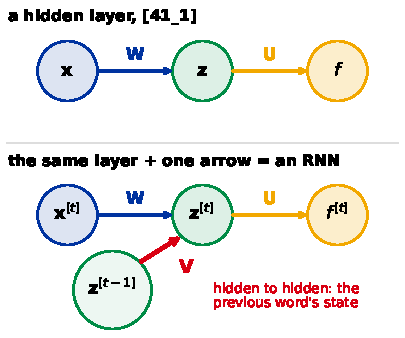
\includegraphics[width=\linewidth]{one_new_arrow.pdf}
    \end{center}
  \end{columns}
\end{frame}

% 2026-10-15 (instructor): the classic folded = unrolled picture was missing; the old
% "Unrolling" click-through below is really an order test and is retitled.
\begin{frame}{Unrolling: one loop, drawn out in time}
  \small
  The red loop says "feed the state back in at the next word". Draw a separate copy of the
  cell for every word and the loop becomes a chain:
  \begin{center}
    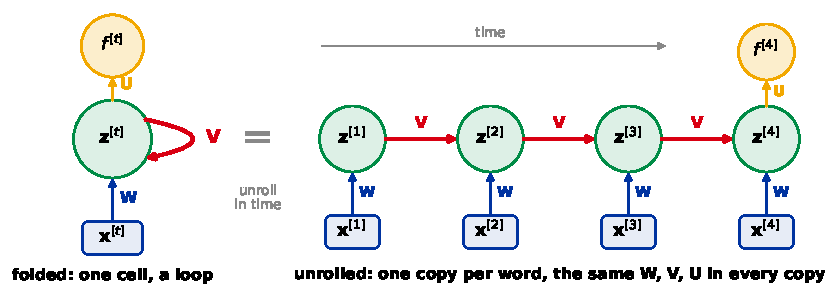
\includegraphics[width=\linewidth]{folded_unrolled.pdf}
  \end{center}
  \vskip -2pt
  \fcolorbox{armblue}{armblue!8}{\parbox{0.97\linewidth}{\raggedright\small
    The copies are not new parameters. A 4-word review and a 40-word review run the same
    cell, so the chain grows with the text while the network does not - that is how an RNN
    fixes the fixed-input problem. For seq-to-one sentiment only the last copy's $f$ is
    used.}}
\end{frame}

\begin{frame}{Anatomy of one RNN step}
  \small Same recurrence, now with concrete numbers to hold onto: a toy vocabulary of
  $3$ words, a $2$-d hidden state. Every arrow below carries its shape, so you always
  know exactly what multiplies what.
  \textbf{Predict:} the one-hot vector $\mathbf{x}^{[t]}$ meets $\mathbf{W}$ - what
  does that product actually pick out?
  \pause
  \vskip 3pt
  \fcolorbox{armorange}{armorange!12}{\parbox{0.97\linewidth}{\small
    It selects ONE column of $\mathbf{W}^\top$ - equivalently, one row of
    $\mathbf{W}$. That row/column IS this word's own vector in $\mathbb{R}^2$ - the
    attention chapter calls it an \textbf{embedding}.}}
  \vskip 4pt
  \begin{center}
    \resizebox{0.98\linewidth}{!}{%
    \begin{tikzpicture}[font=\scriptsize, >=Latex,
        cell/.style={draw, rounded corners, align=center, minimum height=0.85cm,
          minimum width=1.55cm}]
      \node[cell, fill=armblue!10] (x) at (0,0)
        {$\mathbf{x}^{[t]}$\\[1pt] \tiny one-hot $\in\mathbb{R}^3$};
      \node[cell, fill=paramgreen!10] (zprev) at (0,-2.2)
        {$\mathbf{z}^{[t-1]}$\\[1pt] \tiny $\in\mathbb{R}^2$};
      \node[draw, circle, minimum size=0.55cm] (plus) at (2.5,-1.1) {$+$};
      \node[cell, fill=armorange!16, minimum width=1.1cm] (tanh) at (4.4,-1.1) {tanh};
      \node[cell, fill=paramgreen!15] (z) at (6.4,-1.1)
        {$\mathbf{z}^{[t]}$\\[1pt] \tiny $\in\mathbb{R}^2$};
      \draw[->] (x) -- (plus) node[midway, above, sloped] {$\mathbf{W}$ (3x2)};
      \draw[->, armred, very thick] (zprev) -- (plus)
        node[midway, below, sloped] {\textcolor{armred}{$\mathbf{V}$ (2x2)}};
      \node[gray] at (2.5,-2.0) {\tiny $+\,\mathbf{b}$};
      \draw[->, gray] (2.5,-1.75) -- (plus.south);
      \draw[->] (plus) -- (tanh);
      \draw[->] (tanh) -- (z);
      \node[cell, fill=armred!10, dashed, minimum width=1.0cm] (sig) at (8.9,-1.1)
        {$\sigma$};
      \node[cell, fill=armred!14, dashed] (score) at (11.1,-1.1)
        {score\\[1pt] \tiny $\in(0,1)$};
      \draw[->, armorange, dashed] (z) -- (sig)
        node[midway, above, sloped] {\textcolor{armorange}{$\mathbf{U}$ (2x1)}};
      \draw[->, armorange, dashed] (sig) -- (score);
      \node[armorange] at (10.0,-0.15) {\tiny after the last word};
    \end{tikzpicture}%
    }
  \end{center}
\end{frame}

\begin{frame}{A complete forward pass, in real numbers}
  The chapter's Armenian line, first three words, through exactly the net above.
  \textbf{(Click to advance.)}
  \begin{center}
    \only<1>{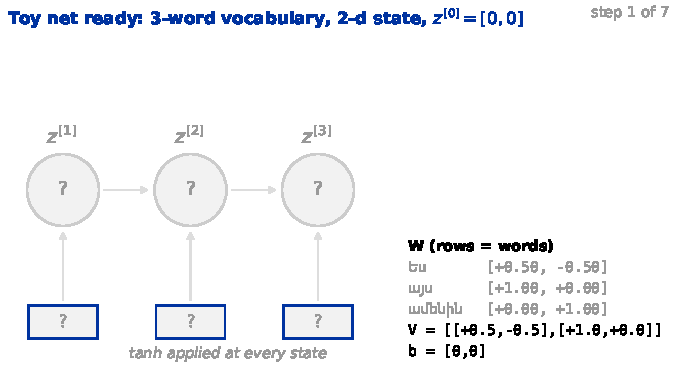
\includegraphics[width=0.82\linewidth]{forward_pass_0.pdf}}%
    \only<2>{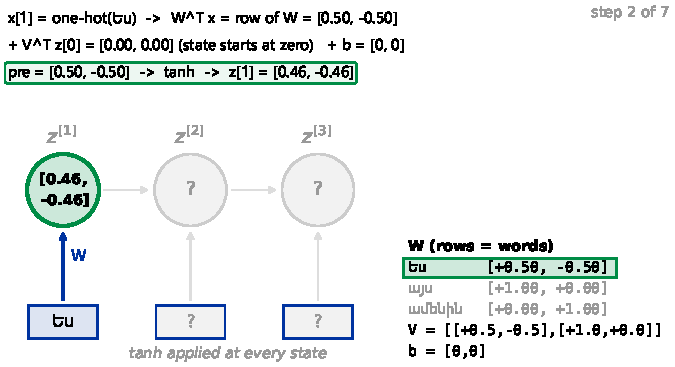
\includegraphics[width=0.82\linewidth]{forward_pass_1.pdf}}%
    \only<3>{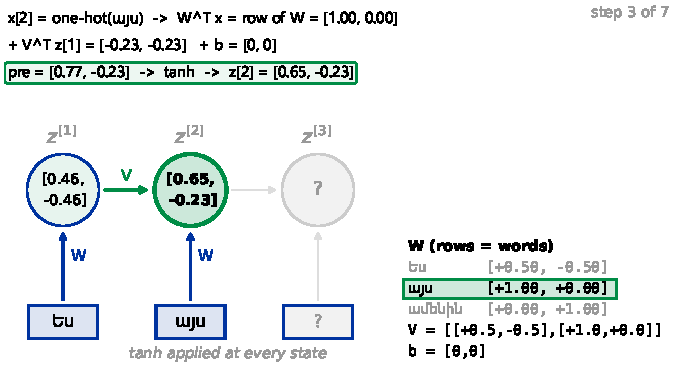
\includegraphics[width=0.82\linewidth]{forward_pass_2.pdf}}%
    \only<4>{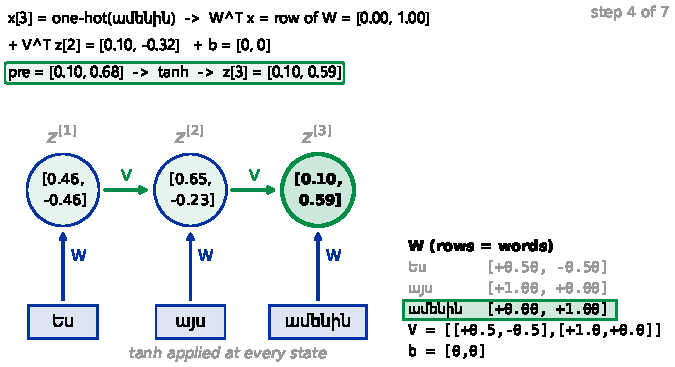
\includegraphics[width=0.82\linewidth]{forward_pass_3.pdf}}%
    \only<5>{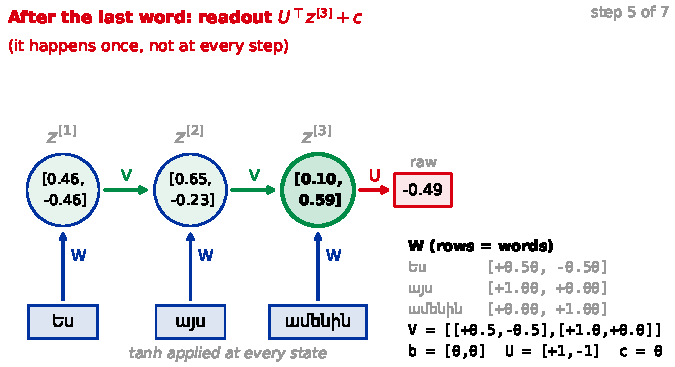
\includegraphics[width=0.82\linewidth]{forward_pass_4.pdf}}%
    \only<6>{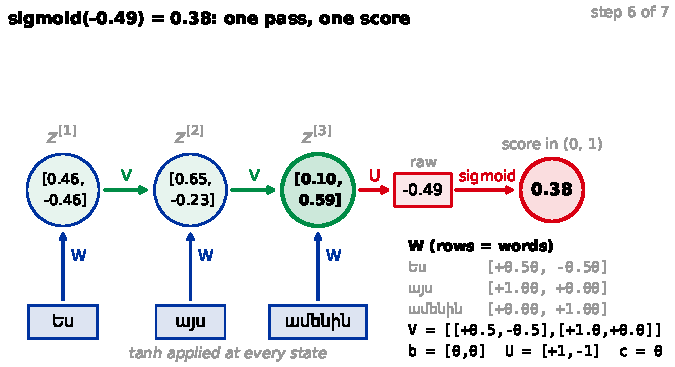
\includegraphics[width=0.82\linewidth]{forward_pass_5.pdf}}%
    \only<7>{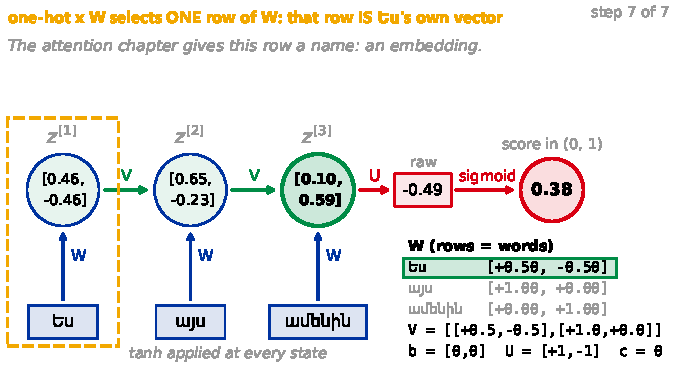
\includegraphics[width=0.82\linewidth]{forward_pass_6.pdf}}%
  \end{center}
\end{frame}

\begin{frame}{Forward pass, summarized}
  \begin{columns}[T]
    \column{0.55\textwidth}
    \small All values rounded to 2 decimals; $\mathbf{z}^{[0]}=[0,0]$, nothing read yet:
    \vskip -3pt
    \begin{align*}
      \mathbf{z}^{[1]} &= \tanh(\mathbf{W}^\top\mathbf{x}_1+\mathbf{b}) = [0.46,-0.46]\\[-1pt]
      \mathbf{z}^{[2]} &= \tanh(\mathbf{V}^\top\mathbf{z}^{[1]}+\mathbf{W}^\top\mathbf{x}_2+\mathbf{b})
        = [0.65,-0.23]\\[-1pt]
      \mathbf{z}^{[3]} &= \tanh(\mathbf{V}^\top\mathbf{z}^{[2]}+\mathbf{W}^\top\mathbf{x}_3+\mathbf{b})
        = [0.10,0.59]\\[-1pt]
      \text{score} &= \sigma(\mathbf{U}^\top\mathbf{z}^{[3]}) = \sigma(-0.49) = 0.38
    \end{align*}
    \column{0.45\textwidth}
    \fcolorbox{popblue}{popblue!6}{\parbox{0.95\linewidth}{\small
      Three words, three applications of the \textbf{same} $\mathbf{W}$ and
      $\mathbf{V}$, one final readout through $\mathbf{U}$. Nothing hidden - every
      number above came straight out of the animation.}}
    \vskip 8pt
    {\footnotesize The weights were set by hand, not trained: $0.38$ is a number to follow,
    not a verdict. In practice $d_h=64$-$512$, not $2$ - but the recipe is identical. And
    it is \textbf{fixed}: 3 words or 3,000, the whole past must fit into those $d_h$
    numbers - a lossy summary [54] will come back to.}
  \end{columns}
\end{frame}

\begin{frame}{Picking the activation: why tanh}
  \begin{columns}[T]
    \column{0.48\textwidth}
    \footnotesize Three candidates for the state's activation - only one is the RNN
    default:
    \begin{itemize}\footnotesize
      \item \textbf{tanh} (default): bounded in $(-1,1)$ - the state literally
        \textbf{cannot blow up} across steps (the state - its gradient still can, as the
        training section shows); zero-centered, so both signs flow.
      \item \textbf{sigmoid}: also bounded, but $|\sigma'|\le 1/4$ everywhere - one
        more shrinking factor on top of $\mathbf{V}$ every step.
      \item \textbf{ReLU}: unbounded above - feed that back through $\mathbf{V}$ every
        step and the state can genuinely \textbf{explode}, not just saturate.
      \end{itemize}
    \vskip 2pt
    \fcolorbox{armred}{armred!8}{\parbox{0.95\linewidth}{\footnotesize
      \textbf{Dead ReLU}, one line: a unit whose pre-activation is always $\le 0$
      outputs zero forever, and its gradient too - it never updates again.}}
    \column{0.52\textwidth}
    \begin{center}
      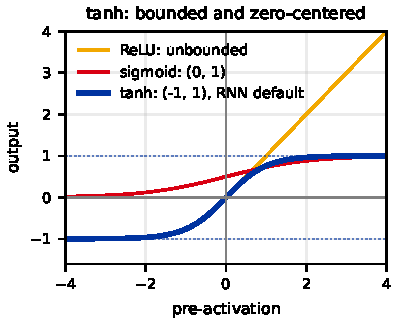
\includegraphics[width=0.92\linewidth]{activation_zoo.pdf}
    \end{center}
  \end{columns}
\end{frame}

\begin{frame}{Same words, different order}
  The \textbf{same} toy net as the forward pass above, same 3 Armenian words - fed
  forward, then fed in the \emph{opposite} order. \textbf{(Click to advance.)}
  \begin{center}
    \only<1>{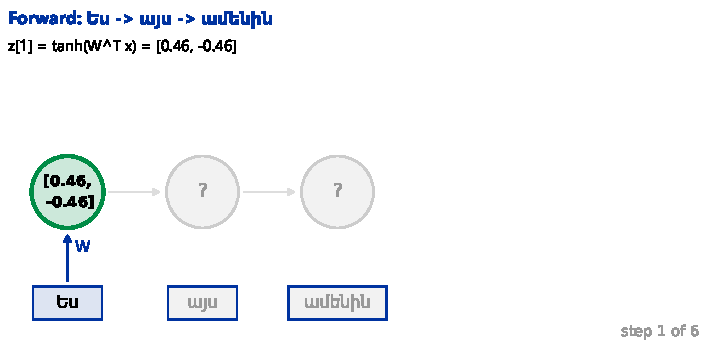
\includegraphics[width=0.86\linewidth]{unroll_0.pdf}}%
    \only<2>{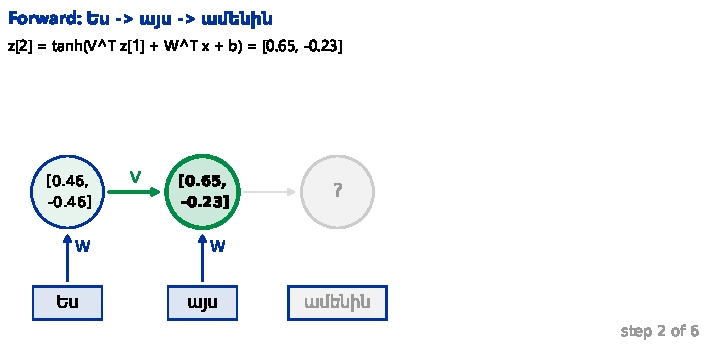
\includegraphics[width=0.86\linewidth]{unroll_1.pdf}}%
    \only<3>{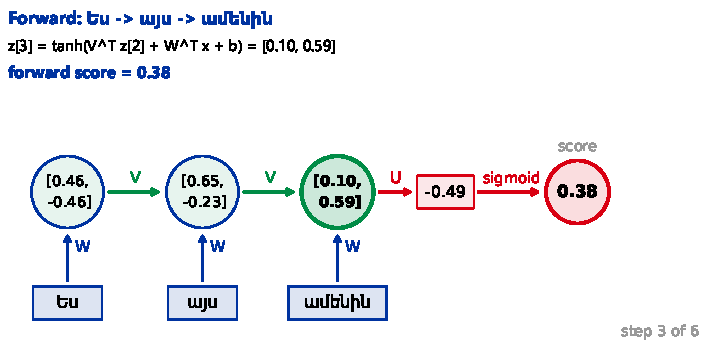
\includegraphics[width=0.86\linewidth]{unroll_2.pdf}}%
    \only<4>{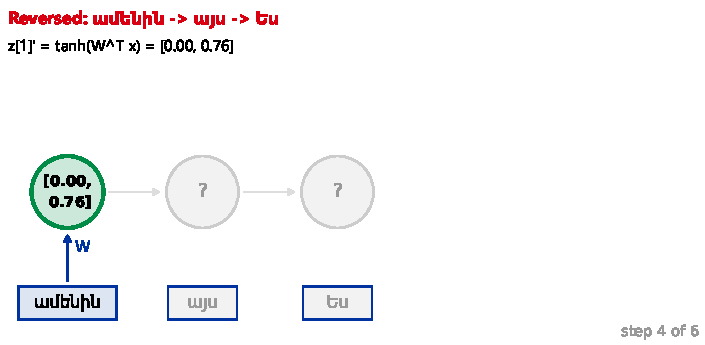
\includegraphics[width=0.86\linewidth]{unroll_3.pdf}}%
    \only<5>{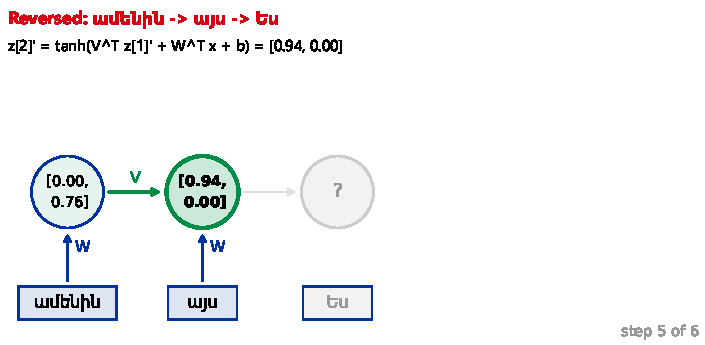
\includegraphics[width=0.86\linewidth]{unroll_4.pdf}}%
    \only<6>{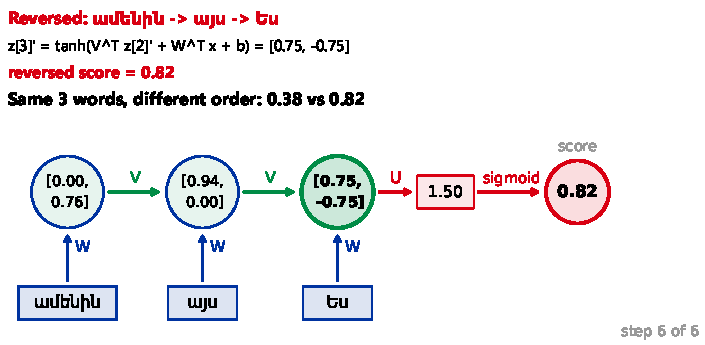
\includegraphics[width=0.86\linewidth]{unroll_5.pdf}}%
  \end{center}
\end{frame}

\begin{frame}{Parameter sharing}
  \begin{columns}[T]
    \column{0.5\textwidth}
    The \emph{same} $\mathbf{W}$ and $\mathbf{V}$ at \textbf{every} step. Parameter
    count is independent of sequence length: with $d_x=1$, $d_h=16$,
    \[
      \underbrace{16}_{W} + \underbrace{256}_{V} + \underbrace{16}_{b}
      + \underbrace{16}_{U} + \underbrace{1}_{c} = \mathbf{305}
    \]
    parameters - whether the review is 3 words or 40.
    \vskip 6pt
    \fcolorbox{armblue}{armblue!8}{\parbox{0.95\linewidth}{\raggedright\small
      Convolution shares across \textbf{space} ([48]); recurrence shares across
      \textbf{time}. Same trick, new axis - and it kills hack (3): a pattern learned at
      position 2 works at position 17 for free.}}
    \column{0.5\textwidth}
    \begin{center}
      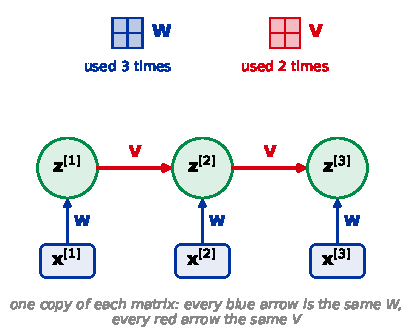
\includegraphics[width=\linewidth]{param_sharing.pdf}
    \end{center}
  \end{columns}
\end{frame}

% 2026-10-15 (instructor): "useful later" - how variable length is handled in a real batch.
% Numbers from py_src/l20_diagrams.py (the locked toy net of forward_pass_anim.py, asserted):
% one zero pad after the 3 words moves the state to [0.56, -0.05] and the score 0.38 -> 0.65.
\begin{frame}{Predict-first: are pads harmless?}
  \begin{columns}[T]
    \column{0.47\textwidth}
    \small
    An RNN reads any length one review at a time. But training runs on \textbf{batches},
    and a batch is a rectangle: every review in it needs the same length. The usual move is
    to fill the short ones with a \texttt{<pad>} token whose input vector is all zeros.
    \vskip 4pt
    \textbf{Predict:} our toy net read the 3 Armenian words and scored $0.38$. Feed it one
    zero \texttt{<pad>} after them. Does the score stay $0.38$?
    \pause
    \vskip 4pt
    \fcolorbox{armred}{armred!8}{\parbox{0.95\linewidth}{\raggedright\small
      No: $\mathbf{0.65}$, and the verdict flips. A zero input is not "nothing": the state
      still goes through $\mathbf{V}$ and tanh,
      $\mathbf{z}^{[4]} = \tanh(\mathbf{V}^\top\mathbf{z}^{[3]} + \mathbf{0} + \mathbf{b})
      = [0.56, -0.05]$. Every pad is one more step of the recurrence.}}
    \column{0.53\textwidth}
    \begin{center}
      \visible<2->{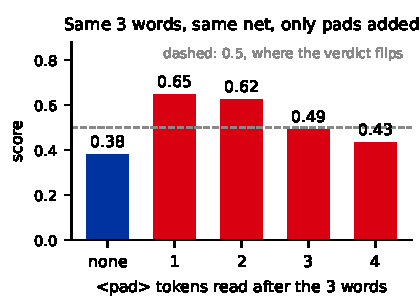
\includegraphics[width=\linewidth]{pad_effect.pdf}}
    \end{center}
  \end{columns}
\end{frame}

\begin{frame}{The fix: pad, then mask}
  \begin{center}
    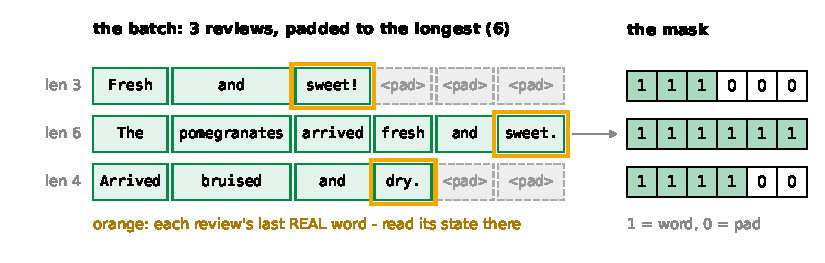
\includegraphics[width=0.86\linewidth]{pad_mask.pdf}
  \end{center}
  \vskip -4pt
  \small
  \begin{itemize}\small
    \item where the 0/1 \textbf{mask} is 0, the state is copied ($\mathbf{z}^{[t]} =
      \mathbf{z}^{[t-1]}$): as if the pad was never read (zeroing it would erase the review);
    \item each review is read at \textbf{its own} last real word, not at column 6;
    \item in next-word prediction, the loss skips the pad positions.
  \end{itemize}
  \vskip 2pt
  \fcolorbox{paramgreen}{paramgreen!8}{\parbox{0.97\linewidth}{\raggedright\footnotesize
    PyTorch: \texttt{pad\_sequence} pads; \texttt{pack\_padded\_sequence(x, lengths)} stops
    each review at its own length. Hugging Face tokenizers return the mask as
    \texttt{attention\_mask} (LLM chapter).}}
\end{frame}

\begin{frame}{The taxonomy}
  \begin{center}
    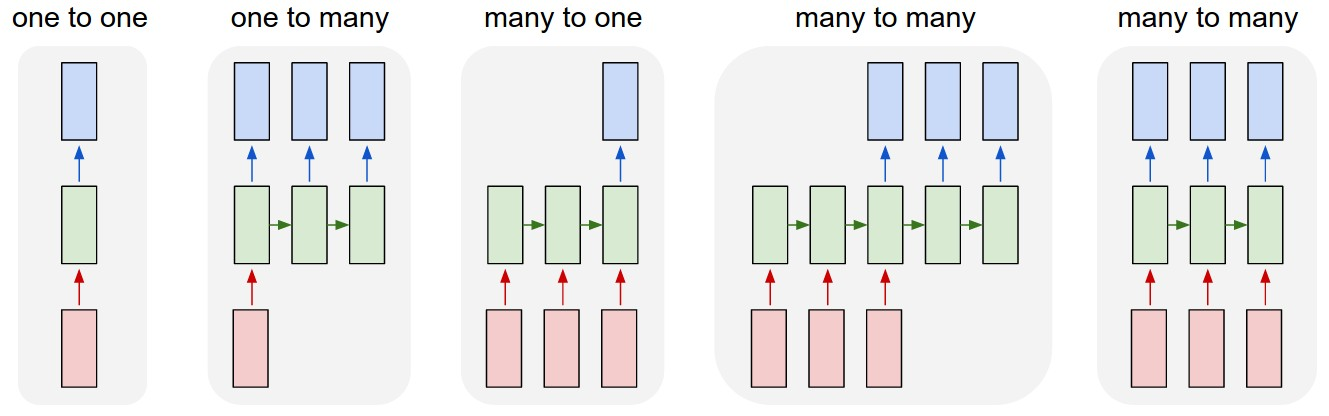
\includegraphics[width=0.76\linewidth]{karpathy_rnn_taxonomy.jpeg}
  \end{center}
  \vskip -2pt
  \begin{itemize}\small
    \item \textbf{seq-to-one}: sentiment (our reviews). One readout, at the end:
      $\sigma(\mathbf{U}^\top\mathbf{z}^{[T]})$.
    \item \textbf{one-to-seq}: image captioning.
    \item \textbf{seq-to-seq, delayed} (4th): translation. Read everything first; then a
      second RNN writes one word per step, each fed back in ([54]).
    \item \textbf{seq-to-seq, synced} (5th): language modeling, tagging. The \emph{same}
      $\mathbf{U}$ reads every state, $\hat{\mathbf{y}}^{[t]} =
      \text{softmax}(\mathbf{U}^\top\mathbf{z}^{[t]})$. $\mathbf{z}^{[t]}$ has seen
      $\mathbf{x}^{[1]}, \dots, \mathbf{x}^{[t]}$, so $\hat{\mathbf{y}}^{[1]}$ knows only
      $\mathbf{x}^{[1]}$. Language model: $\hat{\mathbf{y}}^{[t]}$ guesses
      $\mathbf{x}^{[t+1]}$.
  \end{itemize}
  \vskip 0pt
  {\footnotesize Variants: bidirectional (next slide), stacked. "many-to-X" = our "seq-to-X".
  Diagram: Karpathy (2015), "The Unreasonable Effectiveness of RNNs".\par}
\end{frame}

\begin{frame}{Reading both ways: bidirectional RNNs}
  \begin{columns}[T]
    \column{0.44\textwidth}
    \begin{center}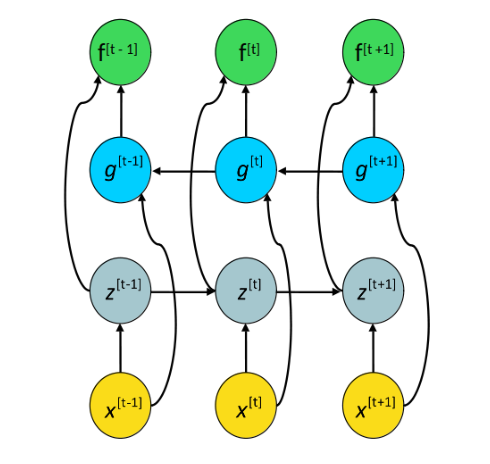
\includegraphics[width=0.84\linewidth]{bidir_rnn.png}\end{center}
    \vskip 1pt
    {\scriptsize The \textbf{forward} states $z^{[t]}$ run left$\to$right; the
    \textbf{backward} states $g^{[t]}$ run right$\to$left; each output $f^{[t]}$ reads
    \emph{both}.}
    \column{0.56\textwidth}
    \small
    A plain RNN only sees the \textbf{past}. But the right reading of a word often depends on
    what comes \emph{after}:
    \vskip 3pt
    \begin{itemize}\small
      \item \emph{``\textbf{Teddy} Roosevelt''} vs \emph{``\textbf{Teddy} bears''} - is
        ``Teddy'' a name? You only know from the \emph{next} word.
    \end{itemize}
    \vskip 4pt
    A \textbf{bidirectional} RNN (Schuster \& Paliwal, 1997) runs one RNN each way and
    concatenates their states, so \textbf{every position sees the whole sequence}.
    \vskip 6pt
    \fcolorbox{armblue}{armblue!8}{\parbox{0.95\linewidth}{\small
      Great for \textbf{encoding} a sequence you already have (tagging, sentiment, the
      encoder half of translation). The catch: it needs the \emph{whole input up front}, so
      it cannot \textbf{generate} or stream token by token - the setting [54] cares about.}}
  \end{columns}
\end{frame}

% ================================================================
\section{Training - and the fatal flaw}

\begin{frame}[plain]
  \vfill
  \begin{center}
    {\Large\color{popblue}\textbf{Training - and the fatal flaw}}\\[0.9em]
    \begin{minipage}{0.82\textwidth}\centering\small
      Unroll it, and it is just a deep network.
    \end{minipage}
  \end{center}
  \vfill
\end{frame}

\begin{frame}{Backprop through time}
  \begin{columns}[T]
    \column{0.46\textwidth}
    \small
    The unrolled RNN is a deep feed-forward net with \textbf{tied weights}: [42]'s
    \texttt{loss.backward()} handles it unchanged. A tied weight collects the \textbf{sum}
    of its gradients from every step, like a shared conv kernel ([48]):
    \[
      \frac{\partial L}{\partial \mathbf{V}} = \sum_{t=2}^{T}
        \frac{\partial L}{\partial \mathbf{V}}\Big|_{\text{use at step } t}
    \]
    For seq-to-one sentiment, $L$ is the log-loss of the final score against the review's
    label, and it sits only at the \textbf{final} step - so its gradient must travel back
    through every recurrent connection.
    \column{0.54\textwidth}
    \begin{center}
      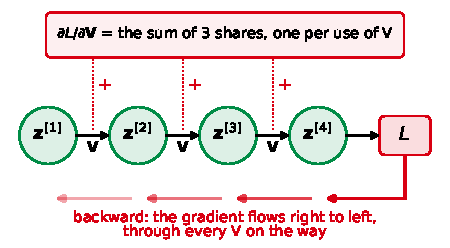
\includegraphics[width=\linewidth]{bptt.pdf}
    \end{center}
    \vskip -2pt
    {\footnotesize Very long texts: backprop through only the last $k$ steps
    (\textbf{truncated} BPTT). Formalized as "backpropagation through time" by Werbos (1990)
    - four years after backprop itself (Rumelhart, Hinton \& Williams, 1986).\par}
  \end{columns}
\end{frame}

\begin{frame}{Predict-first: the fading number}
  \begin{columns}[T]
    \column{0.42\textwidth}
    Strip the net down to $1$-d: a scalar state $h^{[t]}=V h^{[t-1]}+W x^{[t]}$, no
    activation. On a 30-word review, how much does token $1$ influence the state at token
    $30$?
    \[
      \frac{d h_{30}}{d h_1} = V^{29} = 0.8^{29}
    \]
    \textbf{Guess the value.}
    \pause
    \vskip 4pt
    \fcolorbox{armred}{armred!8}{\parbox{0.95\linewidth}{\small
      $0.8^{29}\approx \mathbf{0.0015}$. And if $V=1.25$? $1.25^{29}\approx\mathbf{646}$.
      One multiplication, repeated, either starves or explodes.}}
    \vskip 2pt
    {\footnotesize [29]'s smoothing had the same $0.8$. There, fading is the point; in
    language it is the disease.}
    \column{0.58\textwidth}
    \begin{center}
      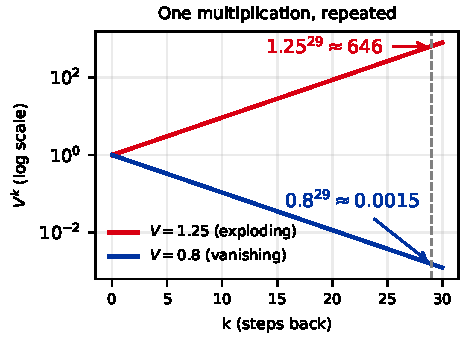
\includegraphics[width=\linewidth]{vanish_curve.pdf}
    \end{center}
  \end{columns}
\end{frame}

% 2026-10-20 (Sonnet student review): the reviewer lost the thread between the scalar 0.8^29
% and "the largest eigenvalue decides". Numbers from l20_diagrams.py fig_eigen_bridge
% (asserted): V = [[1,-0.2],[-0.2,1]], eigenvalues 0.8 / 1.2, |V^29 (1,0)| = 139.9.
\begin{frame}{From one number to a matrix}
  \begin{columns}[T]
    \column{0.47\textwidth}
    \small
    In a real RNN, $\mathbf{V}$ is a matrix. Take a small one:
    \[
      \mathbf{V} = \begin{bmatrix} 1.0 & -0.2 \\ -0.2 & 1.0 \end{bmatrix}
    \]
    No entry is bigger than $1$. \textbf{Predict:} multiply the vector $(1, 0)$ by
    $\mathbf{V}$, 29 times. Does it shrink or grow?
    \pause
    \vskip 4pt
    \fcolorbox{armred}{armred!8}{\parbox{0.95\linewidth}{\raggedright\small
      It grows, to about $\mathbf{140}\times$ its length. $\mathbf{V}$ has two special
      directions, its \textbf{eigenvectors}: along $(1,1)$ it multiplies by $\lambda = 0.8$,
      along $(1,-1)$ by $\lambda = 1.2$. Split $(1,0)$ into those two parts and $\mathbf{V}$
      only rescales each one: $0.8^{29} \approx 0.0015$, $1.2^{29} \approx 198$.}}
    \column{0.53\textwidth}
    \begin{center}
      \visible<2->{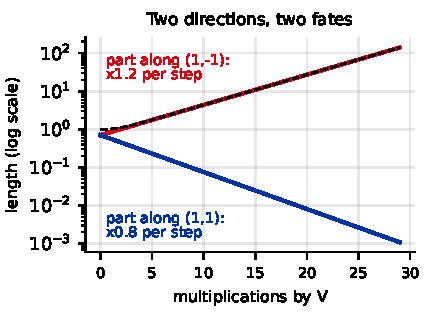
\includegraphics[width=\linewidth]{eigen_bridge.pdf}\\[-2pt]
      {\footnotesize Dashed: the whole vector. After a few steps it \emph{is} the
      $\lambda = 1.2$ part: the largest $|\lambda|$ takes over.}}
    \end{center}
  \end{columns}
\end{frame}

\begin{frame}{The full derivation, part 1}
  For vectors, the state update is
  $\mathbf{z}^{[t]} = \sigma(\mathbf{V}^\top\mathbf{z}^{[t-1]}+\mathbf{W}^\top\mathbf{x}^{[t]}+\mathbf{b})$,
  so by the chain rule:
  \[
    \frac{d\mathbf{z}^{[t]}}{d\mathbf{z}^{[t-1]}}
      = \text{diag}\big(\sigma'(\cdot)\big)\,\mathbf{V}^\top
      = \mathbf{D}^{[t-1]}\,\mathbf{V}^\top
  \]
  Chain this back to step $1$ - one factor per step:
  \[
    \frac{dL}{d\mathbf{z}^{[1]}} = \frac{dL}{d\mathbf{z}^{[t]}}\;
      \mathbf{D}^{[t-1]}\mathbf{V}^\top\,\mathbf{D}^{[t-2]}\mathbf{V}^\top\cdots
      \mathbf{D}^{[1]}\mathbf{V}^\top
  \]
  \vskip 8pt
  \fcolorbox{popblue}{popblue!6}{\parbox{0.97\linewidth}{\raggedright\small
      Every path back to an early time-step multiplies by the \textbf{same} matrix
      $\mathbf{V}^\top$ once per step, $t-1$ times. The $\mathbf{D}$'s sit in between, and
      they never help: $\tanh' \le 1$, so each $\mathbf{D}$ can only shrink a vector. If
      $\mathbf{V}^\top$ alone shrinks every vector, the whole chain shrinks at least as
      fast - the $\mathbf{D}$'s are a bound, not a rescue.}}
  \vskip 6pt
  {\small \textbf{Why eigenvalues?} Along an eigenvector $\mathbf{v}$, the matrix only
  scales: $\mathbf{V}^\top\mathbf{v} = \lambda\mathbf{v}$, so
  $(\mathbf{V}^\top)^{k}\mathbf{v} = \lambda^{k}\mathbf{v}$ - the scalar story again, one
  direction at a time. As in the $2\times 2$ example, after many steps the direction with
  the largest $|\lambda|$ dominates everything else.}
\end{frame}

\begin{frame}{The full derivation, part 2 - eigenvalues}
  The \textbf{largest eigenvalue} $|\lambda_{\max}|$ of $\mathbf{V}$ decides the fate of
  $(\mathbf{V}^\top)^{t-i}$:
  \begin{itemize}
    \item $|\lambda_{\max}| < 1 \Rightarrow$ \textbf{vanishing} - and the $\mathbf{D}$
      factors ($\le 1$ for tanh) can only shrink it further.
    \item $|\lambda_{\max}| > 1 \Rightarrow$ it \textbf{can explode} - unless saturated
      $\mathbf{D}$ factors happen to cancel the growth.
  \end{itemize}
  {\footnotesize (Pascanu, Mikolov \& Bengio, 2013, make it precise: with tanh,
  $|\lambda_{\max}| < 1$ is \emph{sufficient} for vanishing, while $|\lambda_{\max}| > 1$
  is only \emph{necessary} for exploding.)}
  \vskip 6pt
  \fcolorbox{armred}{armred!8}{\parbox{0.97\linewidth}{\small
      \textbf{Worse than a deep MLP.} An MLP multiplies \emph{different} matrices: one
      layer's shrinking can be undone by the next. An RNN multiplies the \textbf{same}
      $\mathbf{V}$ every step, so the same direction shrinks (or grows) every time. Sigmoid
      $\mathbf{D}$'s make it worse ($|\sigma'|\le 1/4$).}}
  \vskip 6pt
  {\footnotesize Callback: [42] already met vanishing gradients in deep MLPs (the
  $\delta$ recursion), and [45] fought them with ReLU and He init. Same disease, worse
  here - it is the \emph{same} matrix every step.}
  \vskip 4pt
  {\footnotesize \textbf{History:} this diagnosis is Hochreiter's 1991 diploma thesis
  (written in German, barely read at the time) and, independently, Bengio, Simard \&
  Frasconi (1994). Remember the name Hochreiter - he returns next lecture with the
  cure.}
\end{frame}

\begin{frame}{Exploding is the easy half}
  \begin{columns}[T]
    \column{0.5\textwidth}
    [44] already gave us the fix for cliffs - \textbf{gradient clipping}: cap the
    gradient's norm at a threshold $h$:
    \[
      \text{if } \|\nabla\| > h:\quad \nabla \leftarrow \frac{h}{\|\nabla\|}\,\nabla
    \]
    \vskip 4pt
    \fcolorbox{armorange}{armorange!12}{\parbox{0.95\linewidth}{\small
      One formula (Pascanu, Mikolov \& Bengio, 2013), solved problem. Exploding
      gradients are the \emph{easy} half of this story.}}
    \column{0.5\textwidth}
    \begin{center}
      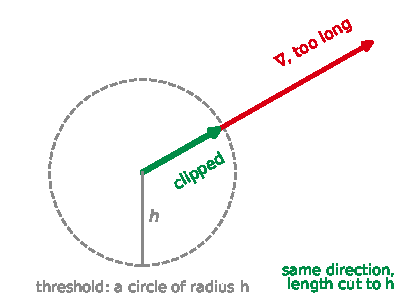
\includegraphics[width=\linewidth]{clipping.pdf}
    \end{center}
  \end{columns}
\end{frame}

% 2026-10-15: the TikZ version drew its formula box and its "cat" box on top of each other;
% redrawn as vanish_practice.pdf (l20_diagrams.py), the formula now in the slide text.
\begin{frame}{What vanishing means in practice}
  \begin{center}
    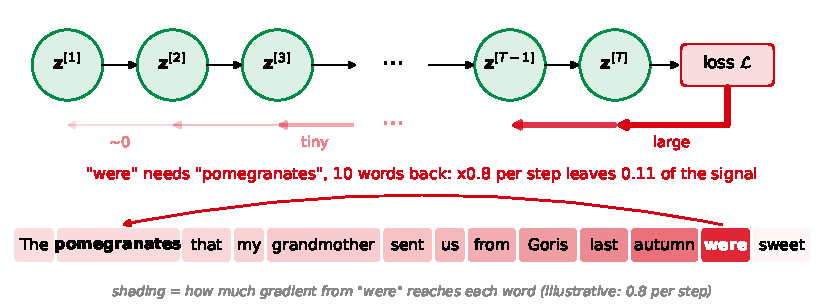
\includegraphics[width=0.96\linewidth]{vanish_practice.pdf}
  \end{center}
  \vskip -4pt
  \small
  $\dfrac{\partial \mathcal{L}}{\partial \mathbf{z}^{[1]}} =
  \dfrac{\partial \mathcal{L}}{\partial \mathbf{z}^{[T]}}
  \cdot \prod_{t=2}^{T} \dfrac{\partial \mathbf{z}^{[t]}}{\partial \mathbf{z}^{[t-1]}}$: a
  product of many factors that shrink, so the gradient vanishes and the RNN \emph{forgets}
  early tokens - here it cannot learn that "were" agrees with "pomegranates".
  \vskip 2pt
  {\footnotesize Our version: the 42-word review from the shoehorn-hacks frame - its
  verdict, \emph{disappointing}, sits in the last clause. By the time the RNN reaches
  it, the state has forgotten most of what came before.}
\end{frame}

\begin{frame}{Empirical proof}
  \begin{columns}[T]
    \column{0.32\textwidth}
    \small
    Gradient norm per time-step, measured directly on a tiny vanilla RNN (hidden size
    $16$). The task: read 30 random numbers, then output the \textbf{first} one - so the
    loss at the end needs the gradient to reach step 1.
    \vskip 6pt
    \fcolorbox{armred}{armred!8}{\parbox{0.95\linewidth}{\small
      \textbf{Read it right to left.} The loss sits at step 29. Each step back keeps
      about \textbf{64\%} of the gradient (log scale: one grid line $= 10\times$). Step 0,
      which holds the answer, gets \textbf{1/350,000} of it.}}
    \column{0.68\textwidth}
    \begin{center}
      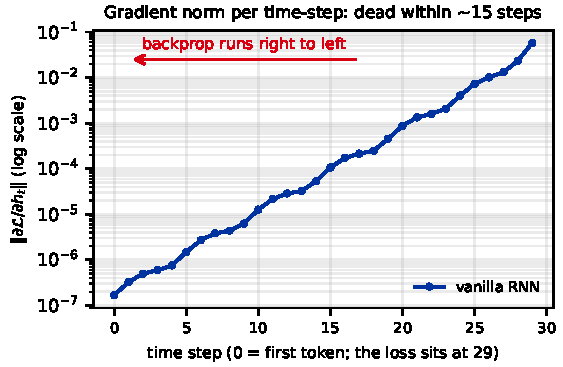
\includegraphics[width=\linewidth]{gradient_flow_vanilla.pdf}
    \end{center}
  \end{columns}
\end{frame}

% ================================================================
\section*{Recap}

\begin{frame}{Recap}
  \begin{itemize}
    \item Text refuses to fit a fixed input: length varies, order matters - every
      shoehorn hack loses one or the other, and a fixed window is blind beyond $k$.
    \item State $=$ a running summary; \textbf{one new weight matrix} $\mathbf{V}$ turns
      a dense layer into an RNN. Batches still need a rectangle: \textbf{pad, then mask}
      - pads are not neutral.
    \item Unrolled $=$ a deep network with \textbf{tied weights} - autograd handles it
      unchanged.
    \item Same-matrix powers $\Rightarrow$ gradients \textbf{vanish} (derived, not
      asserted) or explode.
    \item Clipping fixes exploding. \textbf{Nothing yet fixes vanishing} - so a vanilla
      RNN's "unlimited memory" is, in practice, a few dozen steps: no better than a wide
      fixed window.
  \end{itemize}
  \vskip 6pt
  \fcolorbox{paramgreen}{paramgreen!8}{\parbox{0.97\linewidth}{
      \textbf{Next:} 1997's answer - Hochreiter \& Schmidhuber's \textbf{Long
      Short-Term Memory} (\textbf{LSTM}), a memory built from \textbf{addition}, not
      multiplication. It later runs Google Translate and Siri. And it still will not
      be enough ([54]).}}
\end{frame}

\end{document}

% ================================================================
% Provenance:
%   Deck: L20 RNN Foundations (13_rnns). Built 2026-07-13 from
%   53_rnn_foundations_OUTLINE.md (approved) + RNN_CHAPTER_PLAN.md, following the
%   12_cnn borrowing mechanics and L16_cnn_foundations.tex as the style exemplar.
%
%   Chapter running example (constant for L21 too): the review sentence
%   "The pomegranates arrived fresh and sweet." Short/medium/long shoehorn-hack
%   reviews ("Fresh and sweet!"; "...best I've had since Yerevan."; the 42-word
%   complaint ending "disappointing") are this deck's own text, reused across the
%   shoehorn-hacks frame and the vanishing-gradient frame.
%
%   Sources consulted (REDERIVE, read-only, our own notation z/V/W throughout):
%   LMU I2DL rnn/slides-introduction.tex (motivation, V-weights derivation, unrolled
%   sentiment example, parameter sharing, seq-to-one/one-to-seq/seq-to-seq taxonomy);
%   rnn/slides-backprop.tex (BPTT chain product, D-matrix factors, eigenvalue argument,
%   clipping reference). Credit line on title frame per instructor decision (CC BY 4.0).
%   Gradient-clipping frame phrased as a CALLBACK: L15_training_neural_networks.tex
%   ("Saddles and cliffs -- and how we cope", line ~587) already teaches the identical
%   formula, so L20 cites rather than re-derives it.
%
%   OWN-TEX (per plan's whitelist, ml/preamble.tex macros verified - sampred/warnred
%   both exist but were swapped to armred/armred!8 for in-deck color consistency):
%   the "What vanishing means in practice" frame adapts the vanishing-gradient TikZ from
%   misc/dl4nlp/01_pre_transformer.tex (~lines 477-530), same "cat" sentence, plus our
%   own 42-word-review callback line. The static unrolled-RNN TikZ from the same file
%   (~lines 407-472) was NOT added as a separate frame - the mandatory unroll_anim ANIM
%   already covers unrolling with the locked worked numbers, so a second static diagram
%   would be redundant (logged in 53_DECISIONS.md).
%
%   WEB-IMG: fig/borrowed/karpathy_rnn_taxonomy.jpeg, downloaded from
%   http://karpathy.github.io/assets/rnn/diags.jpeg ("The Unreasonable Effectiveness of
%   Recurrent Neural Networks", Andrej Karpathy, 2015), per standing policy (no
%   licensing caveats needed).
%
%   COPY-IMG: fig/borrowed/bidir_rnn.png = cropped computational-graph figure from LMU
%   I2DL week25 01_introduction.pdf p28 (bidirectional RNN), on the "Reading both ways"
%   frame; no per-image credit line (chapter-level LMU credit on the title frame). Added
%   this session at instructor request, overriding the plan's "bidirectional = one-liner
%   only" scope decision.
%
%   Figures (py_src -> fig, ma venv, seed 509): word_shuffle.pdf (word_shuffle.py, still
%   the English review sentence - see REVISION PASS below for why it was not switched
%   to the Armenian line); pad_truncate.pdf (pad_truncate.py, shared per-column widths so
%   the length-8 boundary lines up across the three review rows); vanish_curve.pdf
%   (vanish_curve.py, 0.8^k vs 1.25^k, log scale); gradient_flow_vanilla.pdf
%   (gradient_flow.py, manual RNNCell/LSTMCell unroll with retain_grad() per step -- a
%   fused nn.RNN call hides the recurrent chain from autograd's exposed gradients, so
%   per-timestep dL/dh_t must be captured this way; also emits
%   gradient_flow_vanilla_lstm.pdf for L21, not used here).
%
%   REVISION PASS (instructor review, this session) added/changed:
%   forward_pass_0.pdf..forward_pass_6.pdf (forward_pass_anim.py, NEW, 7-frame ANIM):
%   the toy 2-d RNN (vocab of 3 words = the Armenian line's first 3 words, W 3x2/
%   V 2x2/b, tanh, U 2x1/sigmoid readout) fed the chapter's real Armenian words with
%   real numbers at every intermediate, read from py_src/data/armenian_line.txt (never
%   retyped). activation_zoo.pdf (activation_zoo.py, NEW): tanh/sigmoid/ReLU curves,
%   tanh highlighted. unroll_0.pdf..unroll_5.pdf (unroll_anim.py, REWRITTEN): now the
%   SAME toy 2-d net and the SAME 3 Armenian words as forward_pass_anim.py (previously
%   a separate 1-d scalar net on the English review words) - narrowed to one
%   punchline, forward vs reversed order giving a different final state AND a
%   different final score (0.38 vs 0.82). Both ANIM scripts promote matplotlib's
%   "Glyph ... missing from current font" warning to a hard error (fail loudly on any
%   future missing-glyph regression) and render Armenian text in Segoe UI (Noto Sans
%   Armenian checked, not installed on this machine; Sylfaen also works).
%
%   Locked worked numbers verified with a throwaway script before typesetting (original
%   build): forward [2,1,3] -> h=[1.0,1.3,2.54]; reversed [3,1,2] -> h=[1.5,1.7,2.36];
%   0.8^29=0.001547; 1.25^29=646.23 (both still used, now only at "Predict-first: the
%   fading number").
%
%   Locked worked numbers (REVISION PASS, toy 2-d net, shared between
%   forward_pass_anim.py and unroll_anim.py - asserted in both scripts):
%   forward z[1]=[0.46,-0.46], z[2]=[0.65,-0.23], z[3]=[0.10,0.59], score=0.38;
%   reversed z[1]=[0.00,0.76], z[2]=[0.94,0.00], z[3]=[0.75,-0.75], score=0.82.
%
%   REVISION 2026-09-06 (instructor request: add historic context, keep the
%   intuition-first focus): added author+year cites - Elman 1990 / Jordan 1986 ("One
%   new arrow"), Werbos 1990 + Rumelhart, Hinton & Williams 1986 ("Backprop through
%   time"), Hochreiter's 1991 diploma thesis + Bengio, Simard & Frasconi 1994 ("The
%   full derivation, part 2" - with the "remember the name Hochreiter" hook to L21),
%   Pascanu, Mikolov & Bengio 2013 (clipping), Schuster & Paliwal 1997
%   (bidirectional), Karpathy 2015 (taxonomy diagram source line). Recap "Next:" box
%   now names Hochreiter & Schmidhuber and expands Long Short-Term Memory (LSTM) on
%   first use. All years web-verified 2026-09-06.
%
%   Key decisions: logged in 53_DECISIONS.md.
%
%   REVISION 2026-09-22 (pre-delivery pedagogy pass, instructor away - autonomous):
%   retired L14/L15 callbacks repointed after checking the delivered decks + their LMU
%   pages: MLP -> [41_2], hidden layer -> [41_1] (LMU uses the same W^T x notation),
%   "the L15 promise" -> [42]'s loss.backward() frame, vanishing gradients in MLPs -> [42]
%   ("What this recursion costs") + [45], clipping -> [44] (LMU 01_challenges: cliffs +
%   gradient clipping). BPTT frame now says a tied weight SUMS its per-step gradients (the
%   rule L16's new shared-kernel frame teaches). NEW frame "What about a fixed window?"
%   between the shoehorn hacks and tokens: L19's 1D conv and the ch11 name inventor
%   (Bengio et al. 2003) both see only the last k tokens; agreement example with the
%   subject 9 words back (Goris). Eigenvalue frame: |lambda| > 1 is only NECESSARY for
%   exploding, |lambda| < 1 SUFFICIENT for vanishing - quoted from Pascanu, Mikolov &
%   Bengio 2013 Sec. 2.1 (arXiv 1211.5063 text), no longer "=> exploding". "Empirical
%   proof" now states the task (read 30 random numbers, output the first) and quotes the
%   measured ratio from logs/gradient_flow.log (2026-07-13 17:48 run, the one plotted):
%   5.82e-2 at t=29 vs 1.70e-7 at t=0 (~340,000x) and 5.36e-5 at t=14 (~1,090x).
%   2026-10-21 (instructor: "i dont get how to read the empirical proof slide"): the box
%   is now a reading guide (right to left; ~64% kept per step back; step 0 gets
%   1/350,000 - the unrounded norms give 348,779, the log's 1.70e-7 is rounded), both
%   asserted in gradient_flow.py --l20-figures; the figure got a "backprop runs right to
%   left" arrow, legend moved to lower right. Taxonomy frame: seq-to-seq split into
%   delayed (4th diagram) and synced (5th), with how each produces its outputs.
%   After a Sonnet student review of the rendered deck (same day): "The full derivation,
%   part 1" now says WHY eigenvalues (along an eigenvector the matrix power is the scalar
%   power); "Forward pass, summarized" says the state is FIXED-size (the lossy summary L21's
%   bottleneck returns to); the recap states the practical consequence - a vanilla RNN's
%   memory is a few dozen steps, no better than a wide window (matches memory_highway.json:
%   RNN at chance on first-token recall by T=80, a coin flip at T=40). Reviewer's proposed
%   cut of the second click-through (Unrolling) NOT applied: instructor-requested revision.
%
%   REVISION 2026-10-03 (instructor review of a proposal list; DECISIONS #64): NEW frame
%   "You have already run a recurrence" - [29]'s simple exponential smoothing
%   (y-hat_{t+1} = alpha y_t + (1-alpha) y-hat_t, notation copied from
%   29_classical_time_series.tex) as the on-ramp to "One new arrow", with a smoothing-vs-RNN
%   table; the 0.8 is paid off in one footnote on "Predict-first: the fading number" ("fading
%   is the point in forecasting, the disease in language"). "One-hot and its poverty" MOVED
%   here from L21 (L21's tokenization section went to the LLM chapter; embeddings are taught
%   there too, so the frame now points forward instead of to an L21 embeddings frame). Stale
%   CNN references after the chapter's move to global numbering: ch6 -> [51], L16 -> [48]
%   (x3), L17 -> [50]. The fixed-window frame's "L19's 1D convolution - a k-token kernel
%   sliding along the text" was wrong twice (1D convolution is taught in [48], on signals,
%   not text) - now "[48]'s 1D convolution, slid along a sentence instead of a signal".
%   Anatomy frame: "next lecture calls it an embedding" -> "the attention chapter".
%   Declined by the instructor in the same review (RNNs stay a quick lecture): a callback to
%   the ch11 name inventor's nn.Embedding, lag features as a third fixed window, a "keep this
%   test" plant on the shuffle frame.
%
%   REVISION 2026-10-03/04 (instructor: "the figures have very small text, e.g. page 17"):
%   every figure redrawn at the size it gets on the slide, fonts 7-10 pt (SLIDE_STYLE.md,
%   Figures). detect_small_figure_text.py: 18 pages under 5.5 pt before, see the commit after.
%   forward_pass_anim.py / unroll_anim.py: drawing code rewritten in inch coordinates at
%   4.5 x 2.45 / 4.7 x 2.3 in (locked matrices, numbers and assertions unchanged); the last
%   forward-pass frame's footnote now says "The attention chapter gives this row a name".
%   word_shuffle.py and pad_truncate.py re-laid out at 3.85 / 5.5 in; pad_truncate now fills
%   the line width (was 0.82) and lists all 34 lost words under the long review.
%   activation_zoo.py, vanish_curve.py, gradient_flow.py resized; gradient_flow.py gained
%   --l20-figures, which reruns the July procedure and checks it reproduces the logged norms
%   before redrawing (1.700e-07 / 5.361e-05 / 5.820e-02 at t = 0 / 14 / 29: reproduced).
%   SPELLING: the chapter line read "ամենինչ"; it is "ամենին" (instructor). Fixed in
%   py_src/data/armenian_line.txt, so the forward-pass and unrolling figures show it.
%
%   Forward pointer: L21 The Road to Attention - LSTM intuition (memory highway = ResNet
%   skip, 18 years earlier), tokenization with the Armenian fragmentation fact, the
%   char-LSTM Armenian generation demo, word embeddings, seq2seq + the bottleneck
%   cliffhanger. gradient_flow_vanilla_lstm.pdf (already generated) is L21's payoff
%   figure for the same toy recall task.
%
%   REVISION 2026-10-15 (instructor review + two rounds of questions; DECISIONS #84):
%   - TikZ -> matplotlib at slot size, new script py_src/l20_diagrams.py: cold_open.pdf (word
%     strips vs an 8-slot input), seq_zoo.pdf (text / speech / music - time series dropped,
%     instructor: "time series was a bad example"), onehot_columns.pdf, onehot_cube.pdf (3 words
%     = 3 cube corners, all sqrt(2) apart, asserted), one_new_arrow.pdf (dense layer vs the same
%     layer + V), param_sharing.pdf, bptt.pdf (dL/dV as a sum of per-use shares - the TikZ
%     arcs had piled onto the nodes), clipping.pdf, vanish_practice.pdf (the TikZ formula box and
%     "cat" box overlapped; the formula is now slide text, the sentence is shaded by 0.8^distance,
%     labelled illustrative). Math labels at 8.5 pt so superscripts stay >= 5.5 pt on the slide.
%   - NEW "Unrolling: one loop, drawn out in time" (folded_unrolled.pdf), the classic picture
%     that was missing; the old "Unrolling" click-through is retitled "Same words, different
%     order" (it is an order test).
%   - NEW "Predict-first: are pads harmless?" (pad_effect.pdf: the locked toy net + one zero pad
%     -> state [0.56, -0.05], score 0.38 -> 0.65; 2-4 pads 0.62 / 0.49 / 0.43, asserted) and
%     "The fix: pad, then mask" (pad_mask.pdf; pad_sequence / pack_padded_sequence checked in the
%     PyTorch 2.13 docs; attention_mask pointer to the LLM chapter). Recap bullet added.
%   - pad_truncate.py: the length-8 line stops at the last row (it ran through the LOST text).
%   - "The full derivation, part 1": the chain was written D...D (V^T)^(t-1), copied from LMU
%     slides-backprop.tex; matrices do not commute, so it is now D V^T D V^T ... D V^T, and the
%     box says it is a pure power only with the D's set to the identity.
%   - Bidirectional image 0.95 -> 0.84 column (its caption sat in the footer band); \raggedright
%     in the narrow callouts (justified text left wide gaps).
%   Detectors after the pass: detect_small_figure_text clean (48 pages), footer collisions 0,
%   clipped 0. Pascanu et al. 2013 re-read for part 2: the paper does say "largest eigenvalue"
%   for the tanh case too, so that footnote stands as written.
%
%   REVISION 2026-10-20 (Sonnet student review of the rendered deck; DECISIONS #92): the
%   reviewer lost the thread at part 1's "with the D's set to the identity" (wording from the
%   10-15 pass). Now: the D's are argued as a bound (tanh' <= 1, each D only shrinks), and a
%   NEW frame "From one number to a matrix" (eigen_bridge.pdf, l20_diagrams.py; asserted:
%   eigenvalues 0.8 / 1.2, |V^29 (1,0)| = 139.9) sits between the 0.8^29 frame and part 1.
%   Also: dL/dV written as a sum over the uses of V, the loss named (log-loss vs the review's
%   label), truncated BPTT in one line (moved under the BPTT figure for room); the mask bullet
%   says why the state is copied, not zeroed; "z[0] = 0, nothing read yet" and "weights set by
%   hand, not trained" on the summary; tanh bounds the state, not its gradient; part 2's MLP
%   comparison said concretely; vanish_practice.pdf uses the Goris sentence (it used "The cat
%   ... was") and z labels (it used h), and the fixed-window frame says 10 words back (the
%   figure asserts the 10 steps). Sigmoid bullet lost its forward reference (overflow).
%   Detectors: small text clean (50 pages), footer collisions 0, clipped 0.
